%*******************************************************************************
%******************************* Final Chapter *********************************
%*******************************************************************************

\chapter{Cosmic $\mu$ Tomography at Wylfa Using Rmon}\label{chp:cosmicMuonTomography}

\ifpdf
    \graphicspath{{Chapter5/Figs/Raster/}{Chapter5/Figs/PDF/}{Chapter5/Figs/}}
\else
    \graphicspath{{Chapter5/Figs/Vector/}{Chapter5/Figs/}}
\fi

\section{$\mu$ Analysis Chain}\label{sec:muonAnalysisChain}
In order to analyse the $\mu$ data from the Wylfa deployment a series of programs called an analysis chain is required. There are two of them for this analysis. The first is based on the T2K analysis chain which converts the data stored in \texttt{.mid.gz} files to \texttt{.root} files and calibrates the data (see figure \ref{fig:mattMurdocksChain}). The second analysis chain (figure \ref{fig:analysisChain}) is designed to analyse simulated data and the data from the upgraded detector once it is complete. However, because the new analysis chain is multi-threaded and much faster in general than the old T2K chain (and isn't dependent on a specific operating system kernel, specific ROOT version and specific GEANT4 version) it is preferable to use the new analysis chain for the Rmon detector data as well. This also has the advantage of ensuring the cosmic $\mu$ tracker will be functional for both versions of the detector (Rmon and VIDARR), allowing for an interesting comparison once the upgraded detector is complete. 
\\\\The Rmon detector deployed at Wylfa analysed data in cycles of 1.5\,$\mu$. There are 23 cycles in the Rmon data from 0 -- 22 with cycle 18 as the trigger cycle and cycles 17 and 19 considered to be underflow and overflow for the trigger signal respectively. The cycles are then interpreted depending on whether the user wants to analyse cosmic $\mu$ data or IBD data. For cosmic $\mu$ data each cycle will be considered as its own event with trigger cycles 17 -- 19 being ignored. Whereas for IBD analysis the data is split between prompt (cycles 0 -- 16) and delayed (cycles 17 -- 19) with the excess data (cycles 20 -- 22) being ignored (see figure \ref{fig:CycleExplaination}). Which mode is decided by the program \texttt{convertOldDetectorData} (see figure \ref{fig:analysisChain}) to ensure the other programs can interpret the Rmon's data correctly. Simulated data requires minimal changes as it puts data into delayed, prompt and ambiguous categories automatically using truth information. Unfortunately, due to the COVID-19 pandemic, the upgraded detector remains incomplete and so the calibration program for the new detector data has not been constructed at present. 

\begin{figure}[!h]
 \centering
 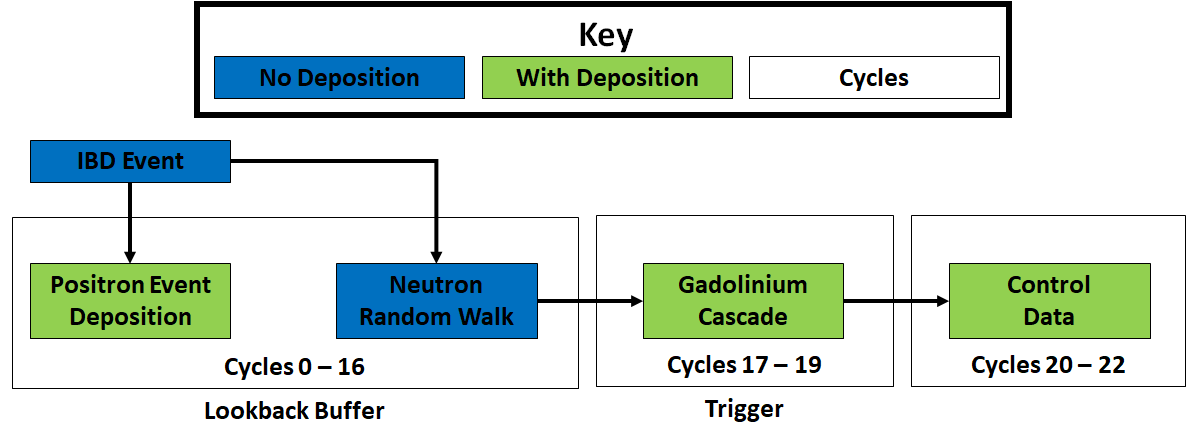
\includegraphics[width=\linewidth]{Chapter6/Figs/CycleExplaination.png}
 \captionof{figure}{The Rmon cycles, the trigger signal is the neutron induced gadolinium cascade in cycle 18 cycles 17 and 19 are overflow. Cycles 0-16 are observed for any signs of a positron cluster as a lookback buffer. Cycles 20-22 contain control information.} 
 \label{fig:CycleExplaination}
\end{figure}

\begin{figure}[!h]
 \centering
 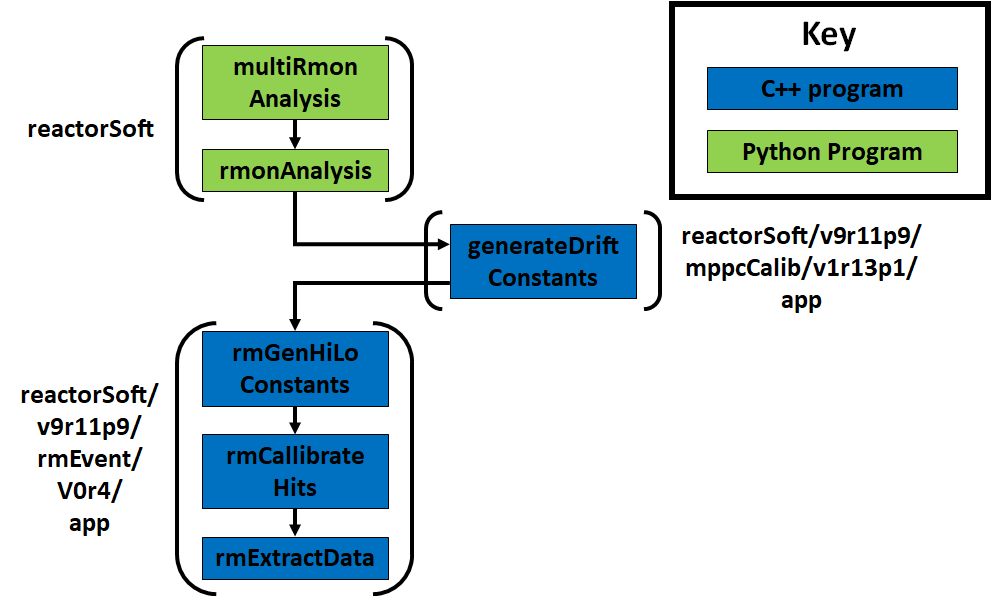
\includegraphics[width=0.8\linewidth]{Chapter5/Figs/Raster/mattMurdocksChain.png}
 \captionof{figure}{The analysis chain for the original detector's .mid.gz files. The python programs are wrappers that control the setup of the software, which programs C++ to run, and the number of instances to run. The C++ programs generate the information needed for calibration and then extract the information to .root files. This is only a small fraction of the analysis chain.} 
 \label{fig:mattMurdocksChain}
\end{figure}
 
\begin{figure}[!h]
 \centering
 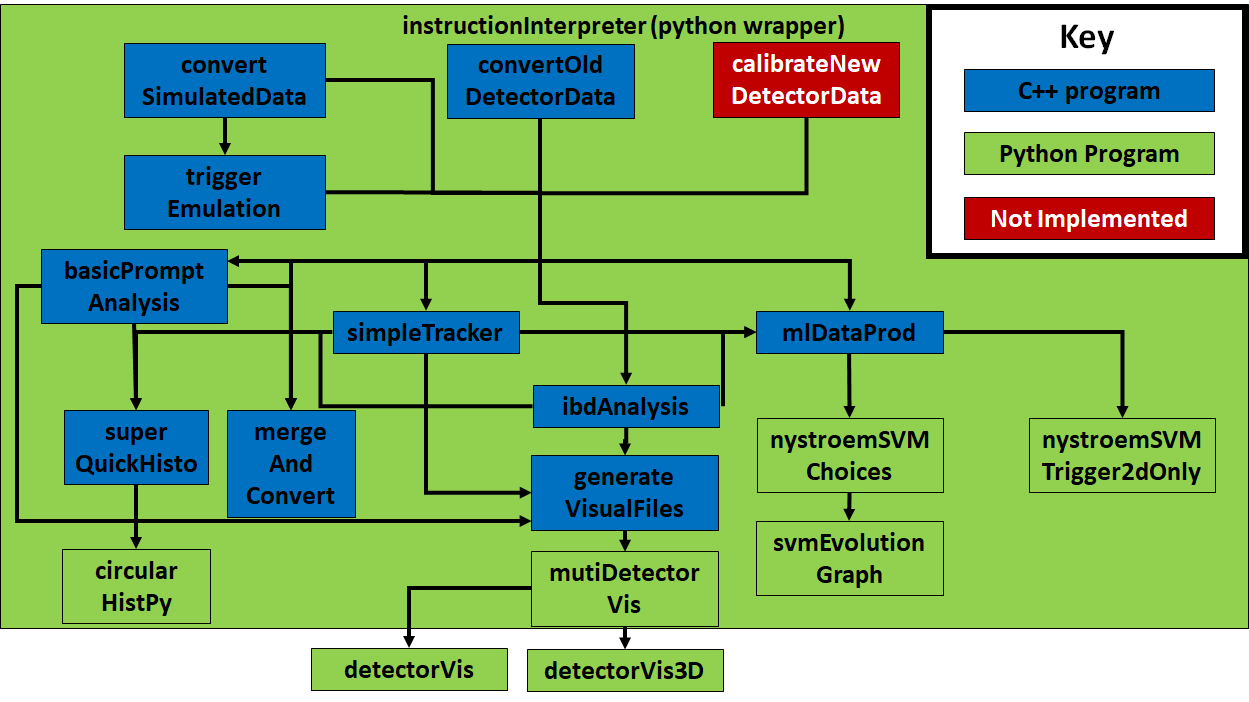
\includegraphics[width=0.8\linewidth]{Chapter5/Figs/Raster/analysisChainRevisedAgain.png}
 \captionof{figure}{The analysis chain for the detector. It is able to process both simulated and measured data. It uses a combination of python programs to handle visualisation and machine learning and C++ programs to process the data. The python program instrutionInterpreter that functions as a wrapper allows for the creation of macro files so results are highly replicable. The C++ programs are multi-threaded. The python programs are in the \textbf{repository} the C++ programs are in \textbf{repository/prg}.} 
 \label{fig:analysisChain}
\end{figure}

The cosmic $\mu$ events at Wylfa were taken in accidental coincidence and as a result, much noise made it into the cosmic $\mu$ data sets. In the raw unprocessed data sets for every 3 cosmic $\mu$ events, there are $\sim$ 10000 noise events. As such the SVM machine learning technique previously described in section \ref{sec:MachineLearningTrigger} was used to filter out the noise. It found the best separating hyper-plane at 8 bars for a threshold of 17.325\,PE (0.693\,MeV) shown in figure \ref{fig:cosmic8BarSignalNoiseCutSVM}.In figure \ref{fig:cosmic8BarSignalNoiseCutSVM}  most of the noise is highly concentrated at a low number of bar hits. As a result, this is a very effective method of removing the noise. This removes 99.9\,\% of noise and keeps 99\,\% of the cosmic $\mu$ signal so now every 3 cosmic events there are $\sim$ 10. The S/N ratio has therefore improved from $\sim$ 3:10000 to $\sim$ 3:10 whilst keeping almost all the signal these numbers are surmised in table \ref{tab:snRatioSvm}. Finding simple effective selection criteria is a task SVMs are well suited to. 

\begin{table*}[!h]
\centering
\begin{tabular}{llll}  
\toprule
Data          & Noise Data\,\% & Signal Data\,\% & S/N Ratio \\
\midrule
Raw Data      & 100            & 100             & $\sim$ 3:10000\\
Data Past SVM & $\sim$ 0.1     & $\sim$ 99       & $\sim$ 3:10\\
\bottomrule  
\end{tabular}
\caption{A table showing how the basic selection criteria }
\label{tab:snRatioSvm}
\end{table*}

\begin{figure}[!h]
\centering
\begin{subfigure}{.5\textwidth}
  \centering
  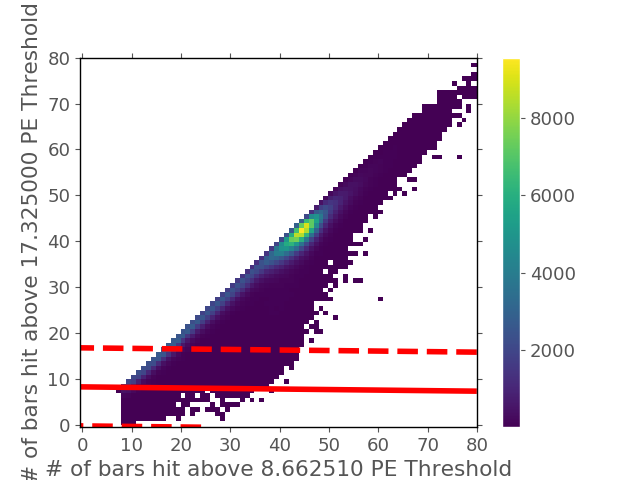
\includegraphics[width=\linewidth]{Chapter5/Figs/Raster/Cosmic8BarSignalCutSVM.png}
  \captionsetup{width=.9\linewidth}
  \caption{}
  \label{subFig:cosmic8BarSignalCutSVM}
\end{subfigure}%
\begin{subfigure}{.5\textwidth}
  \centering
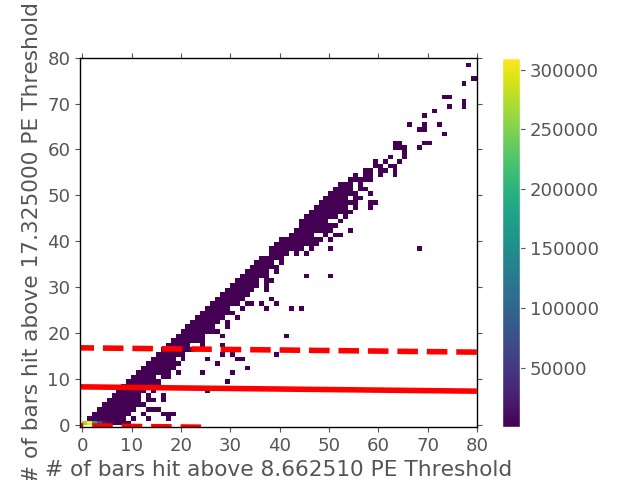
\includegraphics[width=\linewidth]{Chapter5/Figs/Raster/Cosmic8BarNoiseCutSVM.png}
  \captionsetup{width=.9\linewidth}
  \caption{}
  \label{subFig:cosmic8BarNoiseCutSVM}
\end{subfigure}
\caption{How an SVM classifier separates out measured cosmic $\mu$ data it settled on an 8 bar cut above 17.325\,PE (0.693\,MeV). Where everything above the solid line is considered a cosmic $\mu$ and everything below is considered noise. In (a) the $\mu$ data is represented. In (b) the noise data is represented. The logic for the SVM classifier is outlined in figure \ref{sec:MachineLearningTrigger}. }
\label{fig:cosmic8BarSignalNoiseCutSVM}
\end{figure}

% \begin{figure}[!h]
% \centering
% \begin{subfigure}{.5\textwidth}
%   \centering
%   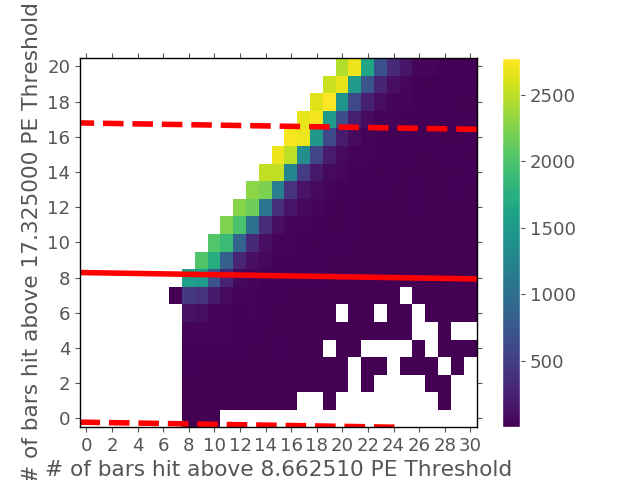
\includegraphics[width=\linewidth]{Chapter5/Figs/Raster/Cosmic8BarSignalZoomCutSVM.png}
%   \captionsetup{width=.9\linewidth}
%   \caption{} 
%   \label{subFig:cosmic8BarSignalZoomCutSVM}
% \end{subfigure}%
% \begin{subfigure}{.5\textwidth}
%   \centering
% 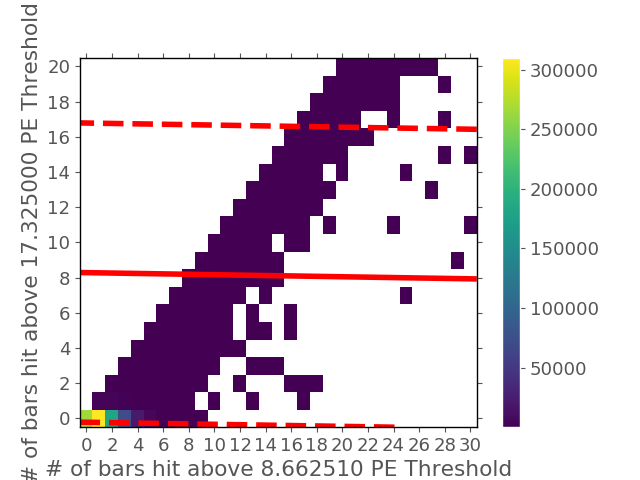
\includegraphics[width=\linewidth]{Chapter5/Figs/Raster/Cosmic8BarNoiseZoomCutSVM.png}
%   \captionsetup{width=.9\linewidth}
%   \caption{}
%   \label{subFig:Cosmic8BarNoiseZoomCutSVM}
% \end{subfigure}
% \caption{Zoomed in version of figure \ref{fig:cosmic8BarSignalNoiseCutSVM} to show how effective the SVM is at removing noise. In (a) the $\mu$ data is represented. In (b) the noise data is represented.}
% \label{fig:Cosmic8BarSignalNoiseZoomCutSVM}
% \end{figure}

In addition, some cycles that contain $\mu$ data are correlated to the trigger cycle 18. These cycles are considered as ``bad'' for cosmic $\mu$ data because they are biased towards the trigger cycles. These bad cycles are shown in figure \ref{fig:badCycles}. Whether a cycle is considered bad depends on whether or not its count rate is above the count rate for cycle 20 in figure \ref{fig:badCycles}. If these bad cycles are added into the data set strange biasing occurs at the side left-hand side of side A and side B as seen in figure \ref{fig:sideABHitsWithBadCycles}. These results are a direct effect of the electronic biasing when taking cosmic $\mu$ data in accidental coincidence and are not a result of track fitting. As will be shown in section \ref{sec:SimulationOfCosmics} the tracker seems to have no obvious biasing associated with it. % as shown later in figures \ref{fig:wylfaSideABHits} and \ref{fig:liverpoolSideABHits} the track fitter does not seem to cause any biasing. 

\begin{figure}[!h]
 \centering
 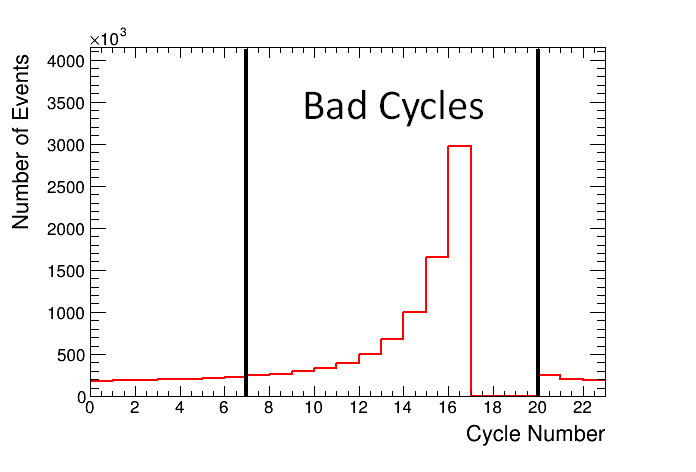
\includegraphics[width=0.7\linewidth]{Chapter6/Figs/badCyclesRedo.png}
 \captionof{figure}{The bad cycles (trigger cycles 17,18 and 19 already removed) for cosmic $\mu$ in the measured data at Wylfa. Whether a cycle is considered ``bad'' depends on how much the cycle correlates to the trigger cycles. I.e. if the count rate extends beyond cycle 20's count rate.} 
 \label{fig:badCycles}
\end{figure}

\begin{figure}[!h]
\centering
\begin{subfigure}{.5\textwidth}
  \centering
  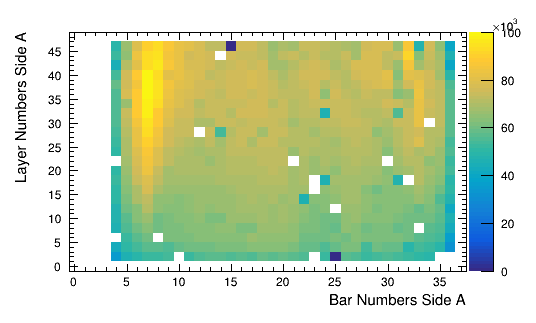
\includegraphics[width=\linewidth]{Chapter5/Figs/Raster/sideAHitsWithBadCycles.png}
  \captionsetup{width=.9\linewidth}
  \caption{} 
  \label{subFig:sideAHitsWithBadCycles}
\end{subfigure}%
\begin{subfigure}{.5\textwidth}
  \centering
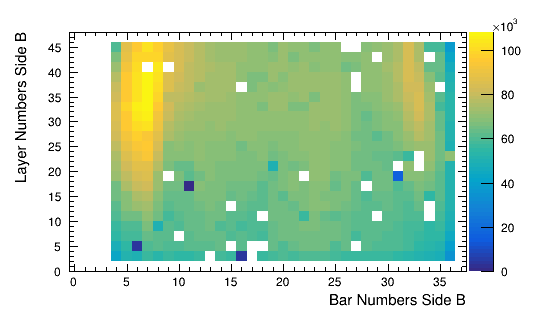
\includegraphics[width=\linewidth]{Chapter5/Figs/Raster/sideBHitsWithBadCycles.png}
  \captionsetup{width=.9\linewidth}
  \caption{}
  \label{subFig:sideBHitsWithBadCycles}
\end{subfigure}
\caption{The detector hits for cosmic $\mu$ when reconstructed with a tracker when bad cycles are included. Side A is shown in (a). Side B is shown in (b). Large streaks are visible on the left-hand sides of both side A and side B.}
\label{fig:sideABHitsWithBadCycles}
\end{figure}

\clearpage
\section{Simulation of Cosmic $\mu$ Hemisphere}\label{sec:SimulationOfCosmics}
% Before the data could be analysed a simulation of cosmic $\mu$ using a cosmic hemisphere was used in order to quantify segmentation and other detector effects. These effects can be quite significant as seen in figures \ref{subFig:phiGenVsRecoHem} and \ref{subFig:cirPhiGenVsRecoHem} the reconstruction of the Rmon detector can be quite adversely affected by vertical events. If an event is vertical in one side of the detector then the other side will dominate as such it results in spikes at $\phi$ = 0$^\circ$, $\phi$ = 90$^\circ$, $\phi$ = 180$^\circ$, $\phi$ = 270$^\circ$. This bin migration is caused by the detector being a segmented cuboid. Any segmented cuboid detector will not cleanly represent a hemispherical distribution. Figures \ref{fig:cosmicBinMigrationSideA} and \ref{fig:cosmicBinMigrationSideB} show how the segmentation of the Rmon/VIDARR detectors cause bin migration. For figure \ref{fig:cosmicBinMigrationSideA} angles of $\phi$ are solely determined by the direction in side A the same is true for side B in figure \ref{fig:cosmicBinMigrationSideB}. 
Any Segmented cuboid detector will not cleanly represent a hemispherical distribution to test the segmentation effect a simulation of cosmic $\mu$ using a cosmic hemisphere was used. If an event is vertical in one side of the detector than the other side will dominate figure  \ref{fig:cosmicBinMigrationSideA} shows an example of what side A dominating event looks like whilst figure \ref{fig:cosmicBinMigrationSideB} shows a side B dominating event. This results in a migration of events at $\phi$ values of $0^\circ$, $90^\circ$, $180^\circ$, and $270^\circ$. This bin migration can be clearly seen in figures \ref{subFig:phiGenVsRecoHem} and \ref{subFig:cirPhiGenVsRecoHem} as the distribution spikes at the expected $\phi$ values. But this segmentation effect is also compounded by the cuboid shape of the detector. In figure \ref{subFig:phiGenVsRecoHem} a clear oscillating pattern can be seen peaking at $\phi$ values of 45$^\circ$, 125$^\circ$, 275$^\circ$, 315$^\circ$ in the reconstructed which is not present in the generated. This is a result of the cuboid shape of the detector. These bin migrations are not a significant concern provided they are properly understood, but it does mean that the data in $\phi$ will be significantly distorted.  
 
\begin{figure}[!h]
 \centering
 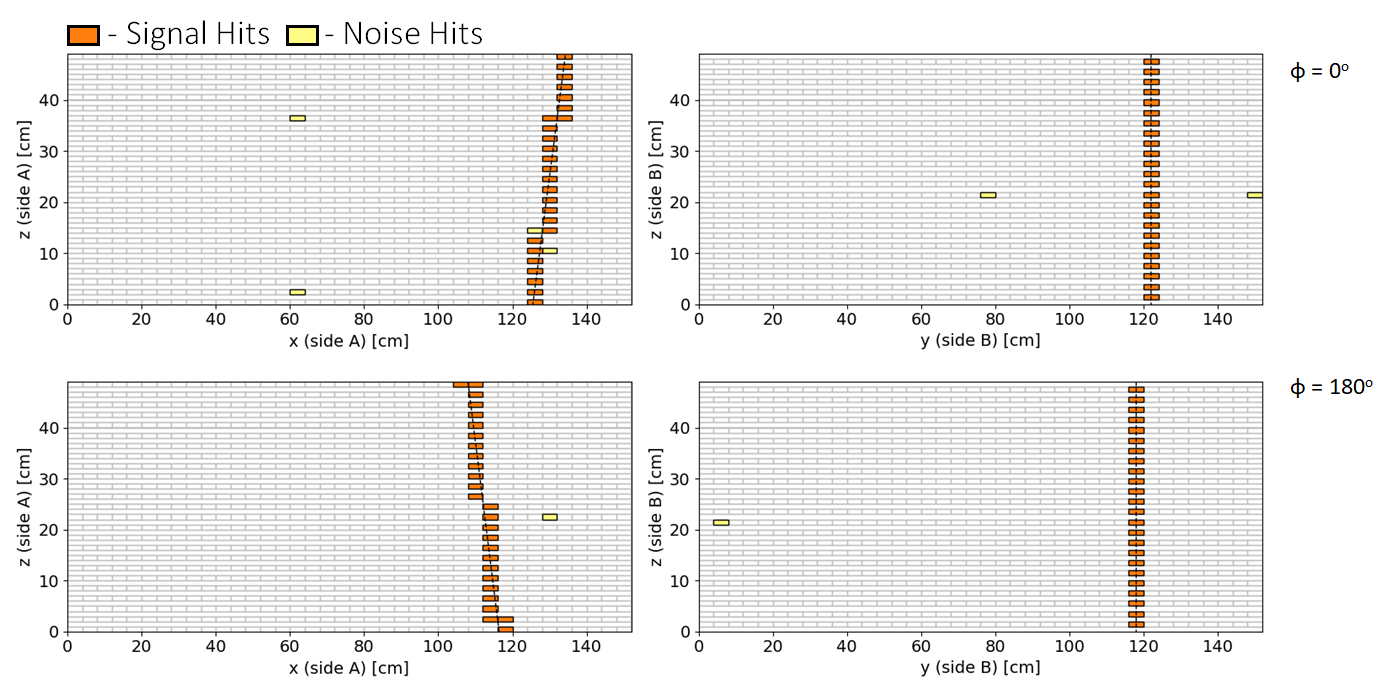
\includegraphics[width=\linewidth]{Chapter6/Figs/phiSideABinMigration.png}
 \captionof{figure}{Side A Bin migration due to the segmentation size of Rmon/VIDARR. In this example side B has no $\phi$ component and so any value on side A determines $\phi$ exclusively warping the distribution.} 
 \label{fig:cosmicBinMigrationSideA}
\end{figure}

\begin{figure}[!h]
 \centering
 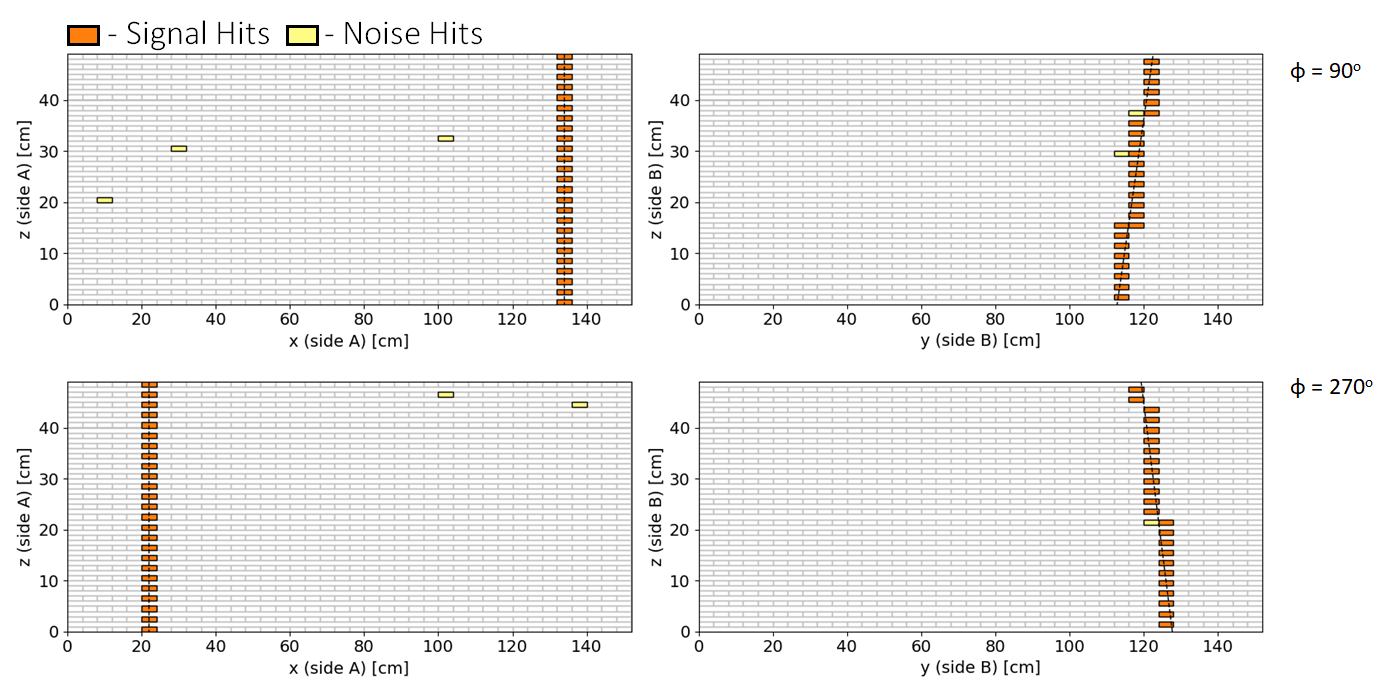
\includegraphics[width=\linewidth]{Chapter6/Figs/phiSideBBinMigration.png}
 \captionof{figure}{Side B Bin migration due to the segmentation size of Rmon/VIDARR. In this example side A has no $\phi$ component and so any value on side B determines $\phi$ exclusively warping the distribution.} 
 \label{fig:cosmicBinMigrationSideB}
\end{figure}

\begin{figure}[!h]
\centering
\begin{subfigure}{.5\textwidth}
  \centering
  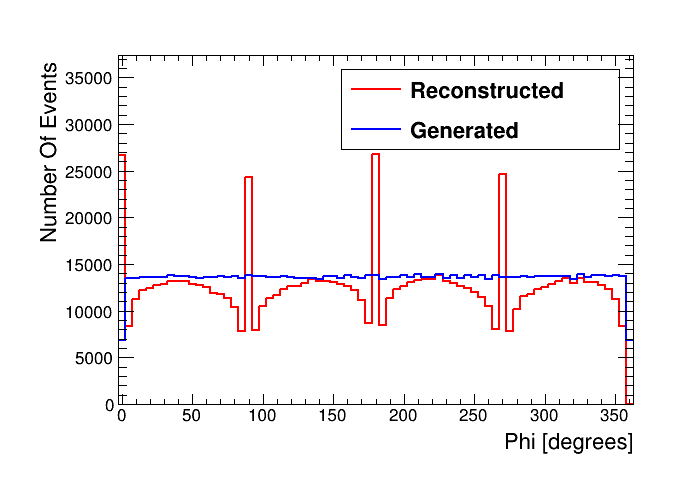
\includegraphics[width=\linewidth]{Chapter6/Figs/hemispherePhi_linHist.png}
  \captionsetup{width=.9\linewidth}
  \caption{} 
  \label{subFig:phiGenVsRecoHem}
\end{subfigure}%
\begin{subfigure}{.5\textwidth}
  \centering
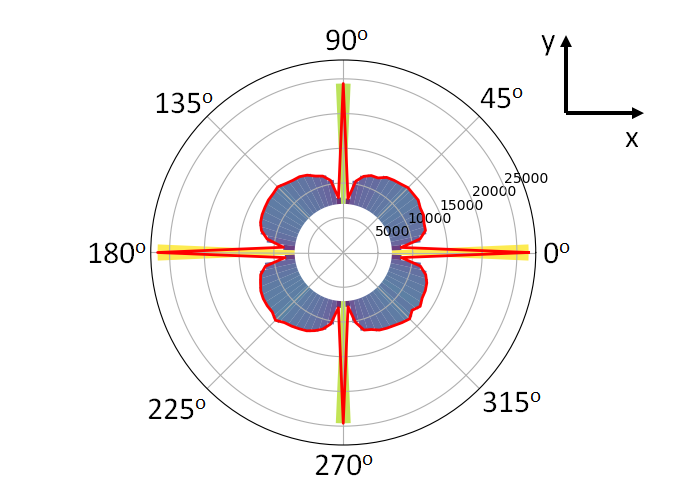
\includegraphics[width=\linewidth]{Chapter6/Figs/hemispherePhi_cirHist.png}
  \captionsetup{width=.9\linewidth}
  \caption{}
  \label{subFig:cirPhiGenVsRecoHem}
\end{subfigure}
\caption{(a) Generated $\phi$ vs reconstructed $\phi$ with the online track fitter for a cosmic hemisphere distribution.(b) Circular plot of the reconstructed $\phi$ for a simulated cosmic hemisphere.}
\label{fig:linCirPhiGenVsRecoHem}
\end{figure}

\clearpage
However, bin migration is significantly less pronounced in $\theta$. As shown by figure \ref{fig:thetaGenVsRecoHem} significant bin migration is is only seen in binned $\theta$ values of 0$^\circ$, 5$^\circ$, 80$^\circ$, 85$^\circ$, 90$^\circ$ but bins 10$^\circ$ -- 75$^\circ$ are accurately reconstructed. The large discrepancy in bin migration between $\phi$ and $\theta$ is due to the size of the segments in the Rmon/VIDARR detectors. The segments are 4\,cm wide by 1\,cm tall so they are able to more accurately reconstruct information vertically than in any other direction. Which is useful for reconstructing vertical information such as the height of buildings. Though as will be outlined in section \ref{sec:cosmicTrackerUncertainties} the segmentation and effect of corner clipping events makes reconstruction of $\theta$ more difficult than expected. When comparing the generated hits for a cosmic hemisphere (figure \ref{fig:rawHemisphereFiducialBarsSideAB}) to the reconstructed hits (figure \ref{fig:HemisphereFiducialBarsSideAB}) they appear to match closely. Therefore, it is reasonable to assume that the tracker does not introduce any biases into the generated data set.

\begin{figure}[!h]
 \centering
 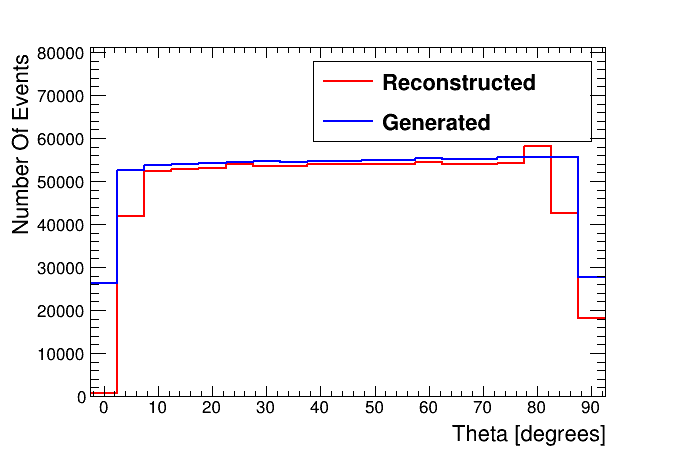
\includegraphics[width=0.6\linewidth]{Chapter5/Figs/Raster/hemisphereThetaCompare.png}
 \captionof{figure}{Generated $\theta$ vs reconstructed $\theta$ for a cosmic hemisphere distribution} 
 \label{fig:thetaGenVsRecoHem}
\end{figure}

\begin{figure}[!h]
\centering
\begin{subfigure}{.5\textwidth}
  \centering
  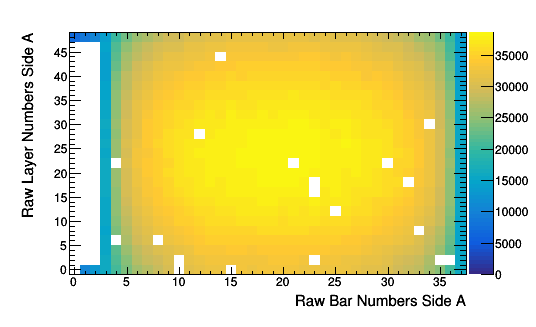
\includegraphics[width=\linewidth]{Chapter5/Figs/Raster/rawHemisphereFiducialBarsSideA.png}
  \captionsetup{width=.9\linewidth}
  \caption{}
  \label{subFig:rawHemisphereFiducialBarsSideA}
\end{subfigure}%
\begin{subfigure}{.5\textwidth}
  \centering
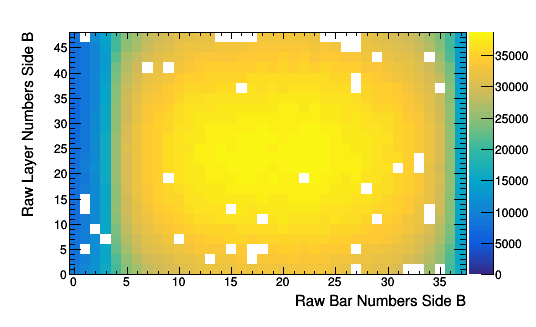
\includegraphics[width=\linewidth]{Chapter5/Figs/Raster/rawHemisphereFiducialBarsSideB.png}
  \captionsetup{width=.9\linewidth}
  \caption{}
  \label{subFig:rawHemisphereFiducialBarsSideB}
\end{subfigure}
\caption{Generated hemisphere bars hit when using the generated $\phi$ seen in figure \ref{subFig:phiGenVsRecoHem} and generated $\theta$ seen in figure \ref{fig:thetaGenVsRecoHem}. Dead and un-instrumented channels are simulated to improve accuracy and the simulation bounds match the fiducial bounds. Side A is shown in (a). Side B is shown in (b).}
\label{fig:rawHemisphereFiducialBarsSideAB}
\end{figure}

\begin{figure}[!h]
\centering
\begin{subfigure}{.5\textwidth}
  \centering
  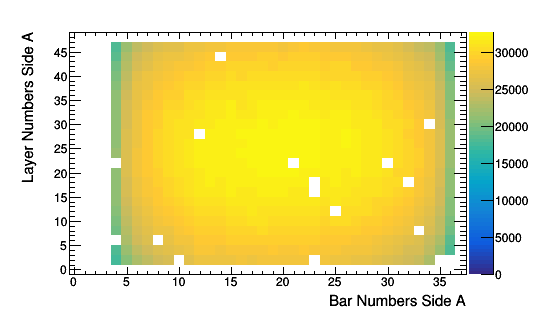
\includegraphics[width=\linewidth]{Chapter5/Figs/Raster/hemisphereFiducialBarsSideA.png}
  \captionsetup{width=.9\linewidth}
  \caption{}
  \label{subFig:hemisphereFiducialBarsSideA}
\end{subfigure}%
\begin{subfigure}{.5\textwidth}
  \centering
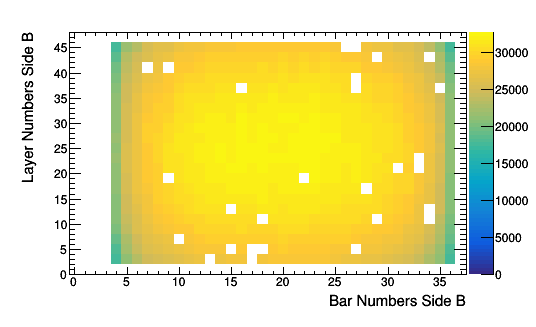
\includegraphics[width=\linewidth]{Chapter5/Figs/Raster/hemisphereFiducialBarsSideB.png}
  \captionsetup{width=.9\linewidth}
  \caption{}
  \label{subFig:hemisphereFiducialBarsSideB}
\end{subfigure}
\caption{Reconstructed hemisphere bars hit when using the reconstructed $\phi$ seen in figure \ref{subFig:phiGenVsRecoHem} and reconstructed $\theta$ seen in figure \ref{fig:thetaGenVsRecoHem}. The tracker is not disrupted by the dead channels and accurately reconstructs the hits seen in figure \ref{fig:rawHemisphereFiducialBarsSideAB} with minimal detector corner clipping events removed. Side A is shown in (a). Side B is shown in (b).}
\label{fig:HemisphereFiducialBarsSideAB}
\end{figure}

The cosmic hemisphere distribution was chosen as it covers all possible angles in the ($\phi$,$\theta$) space that the detector will encounter. When reconstructing the ($\phi$,$\theta$) distribution of the cosmic hemisphere (figure \ref{fig:simulatedHemisphereDist}) a clear bin migration is visible. The reconstruction artefacts are shown in figures \ref{subFig:phiGenVsRecoHem} and \ref{fig:thetaGenVsRecoHem} can be seen to have a dependence on one another in figure \ref{fig:simulatedHemisphereDist}. Apart from the uncertainties introduced from the segmentation and shape of the detector no other uncertainties are significantly visible in figure \ref{fig:simulatedHemisphereDist}. However, this does not mean that other uncertainties are not present just that the most noticeable uncertainty is due to the segmentation and shape of the detector. 

\clearpage
For positional reconstruction, showers are kept but for online use where calibration is the goal showers are discarded. In this analysis, the reconstruction is optimised for the angle-of-incidence extraction (both $\phi$ and $\theta$) as the key analysis variable. The reconstruction steps for fitting each individual track are as follows: 
\begin{enumerate}
  \item \textbf{Remove Small Events:} If < 8 are hit above a threshold of 0.693\,MeV discard that event (see figure \ref{fig:cosmic8BarSignalNoiseCutSVM})
  \item \textbf{Energy Threshold:} Exclude all hits below 0.345\,MeV
  \item \textbf{Track Width:} Exclude hits that are 4 bars away from any other hit 
  \item \textbf{Hit Threshold:} Exclude events that have $<$ 4 bars per side that are above a 0.69\,MeV threshold
  \item \textbf{Basic Fit:} Find a basic gradient and intercept using top and bottom hit of the event
  \item \textbf{First Fit:} First fit of the track 
  \item \textbf{Track Width 2:} Exclude hits that are 4.5 bars away from the track
  \item \textbf{Second Fit:} second fit of the track
  \item \textbf{Track Width 3:} Exclude any hits that are 0.5 bars away from the track
  \item \textbf{Third Fit:} Third and final fit of the track
  \item \textbf{Exclude Bad Events:} Events that have < 50\,\% of the total energy as signal energy are removed
  \item \textbf{Exclude Empty Events:} Any Events that have no signal energy are removed (used if other cuts are disabled) 
\end{enumerate}
The fitter uses the GNU scientific library simplex minimiser \cite{galassi2002gnu} in order to solver for $y = mx + c$ for each side. The minimiser tries to minimise the value of a pseudo $\chi^2$. The $\chi^2$ is approximated by adding (y$_\textrm{{Data}}$ y$_\textrm{{Prediction}}$)$^4$ to the pseudo $\chi^2$ when (y$_\textrm{{Data}}$ y$_\textrm{{Prediction}}$)$^2$ < 1 and adding (y$_\textrm{{Data}}$ y$_\textrm{{Prediction}}$)$^2$ to the pseudo $\chi^2$ otherwise. The quartic function (y$_\textrm{{Data}}$ y$_\textrm{{Prediction}}$)$^4$ is used when predictions are accurate to give a flatter function to fit as its more ``bar like.'' Using this pseudo $\chi^2$ to discriminate against poorly fitted events is tempting. But when trailing this in figure \ref{fig:dedxGenVsRecoHem} there is no approachable difference even though $\sim$ 90\,\% the worst fitted events are removed. As a result for calibration purposes the minimum number of bars to be considered would likely be increase from 8 to 40 to speed up fitting. If this is even required at all, as the tomographic tracker is very fast as will be discussed later. 
% When reconstructing the ($\phi$, $\theta$) space there is no $\chi^2$ discrimination. This is because many cosmic $\mu$ may shower when inside the detector and as a result may have a high $\chi^2$ but are still an accurate representation of cosmic $\mu$ direction. But a $\chi^2$ cut is effective when trying to accurately measure the $dE/dx$ as seen in figure \ref{fig:dedxGenVsRecoHem}. Showers produce many secondaries in the detector which when divided by the same length causes an increase in $dE/dx$ as shown by figure \ref{fig:dedxGenVsRecoHem}. This is because more energy is produced in a track's length than the energy deposited by the MIP like cosmic. As mentioned previously this analysis includes showering events to give as many statistics as possible. a $\chi^2$ cut would be useful for calibration as the $dE/dx$ of cosmic $\mu$ MIPs with no secondaries are useful for calibration. The $\chi^2$ discrimination would be the 10$^{th}$ step. The fitter uses the GNU scientific library simplex minimiser \cite{galassi2002gnu} in order to solve for $y$ = $mx$ + $c$.  

\begin{figure}[!h]
\centering
\begin{minipage}{.45\textwidth}
  \centering
  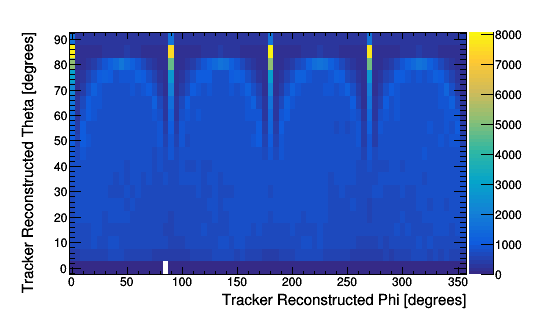
\includegraphics[width=\linewidth]{Chapter5/Figs/Raster/pvsTFiduicalHemisphere.png}
  \captionof{figure}{Simulated cosmic hemisphere which has a flat distribution in $\theta$ from 0$^\circ$ to 90$^\circ$ and a flat distribution in $\phi$ from 0$^\circ$ to 360$^\circ$ which is then reconstructed using the track fitter logic described in section \ref{sec:SimulationOfCosmics}}
  \label{fig:simulatedHemisphereDist}
\end{minipage}%
\qquad
\begin{minipage}{.45\textwidth}
  \centering
  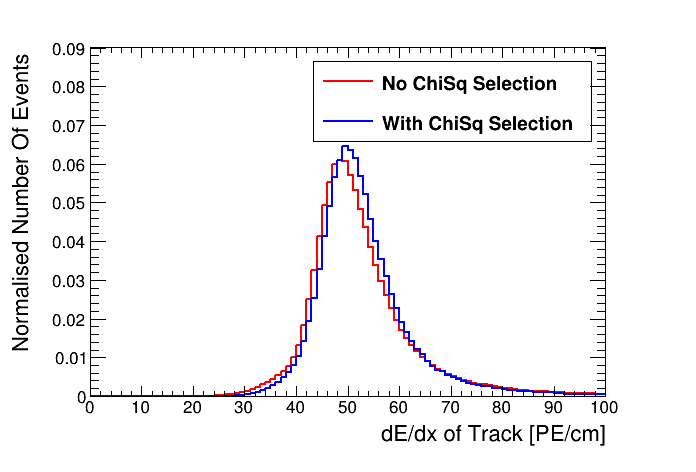
\includegraphics[width=\linewidth]{Chapter6/Figs/simHemDeDx.png}
  \captionof{figure}{dE/dx Of the simulated cosmic hemisphere both with and without a $\chi^2$/DOF selection criteria. Selection removes 90\,\% of events. The difference is minimal suggesting that a good series of selection criteria have been found regardless of $\chi^2$/DOF.}
  \label{fig:dedxGenVsRecoHem}
\end{minipage}
\end{figure}

% \begin{figure}[!h]
%  \centering
%  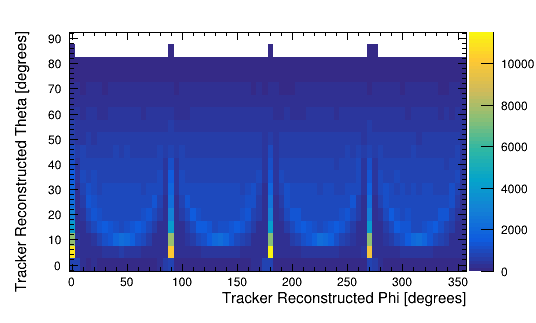
\includegraphics[width=0.8\linewidth]{Chapter5/Figs/Raster/simulatedNormalDistirbution.png}
%  \captionof{figure}{\hl{theta has been reversed now!!!} Simulated distribution with an ideally generated cosmic distribution.} 
%  \label{fig:simulatedNormalDist}
% \end{figure}

\section{Deployment At Wylfa}\label{sec:deploymentAtWylfa}
The Rmon detector was deployed at the Wylfa Nuclear power station from 07-07-2014 to 25-02-2016 with data being taken continuously over that time period both with the reactor on and reactor off taking the IBD measurements seen in figure \ref{fig:prototypeMeasumentFlux}. The placement of the detector in relation to the Wylfa reactor buildings can be seen in figure \ref{subFig:DetectorPositionTopDown}, the reactors are located at either end of the main reactor building the ``dog bone'' and are assumed to be in the centre of the cylinders. Whilst there is no good height data for the buildings at the Wylfa reactor site there is a drone picture available seen in figure \ref{subFig:wylfaArielView}. In figure \ref{subFig:wylfaArielView} the tallest buildings are clearly visible, of particular importance is the main reactor building and the turbine hall. The service buildings in between the turbine hall and the  main reactor building are also very important as they are much closer to the detector's position as seen in figure \ref{subFig:DetectorPositionTopDown} and so will appear taller than the main reactor building. Also in figures \ref{subFig:DetectorPositionTopDown} and \ref{subFig:wylfaArielView} the steam bridges that connect the main reactor building and the turbine hall are also visible. The steam bridges are not large buildings and are approximated to be 5\,m thick and 10\,m off of the ground in simulation. But one of the steam bridges is very close to the detector as can be seen in figure \ref{subFig:DetectorPositionTopDown} and so will occlude a significant portion of the ($\phi$, $\theta$) space the detector observes. 

\begin{figure}[!h]
\centering
\begin{subfigure}{.5\textwidth}
  \centering
  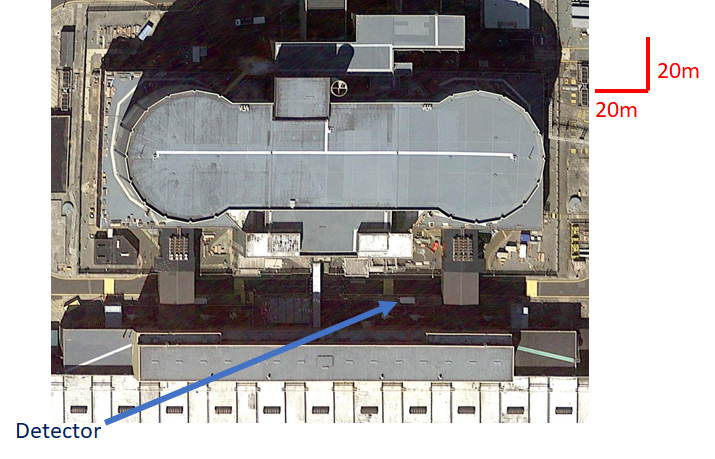
\includegraphics[width=\linewidth]{Chapter5/Figs/wylfaRasterNew/DetectorPositionTopDown.png}
  \captionsetup{width=.9\linewidth}
  \caption{}
  \label{subFig:DetectorPositionTopDown}
\end{subfigure}%
\begin{subfigure}{.5\textwidth}
  \centering
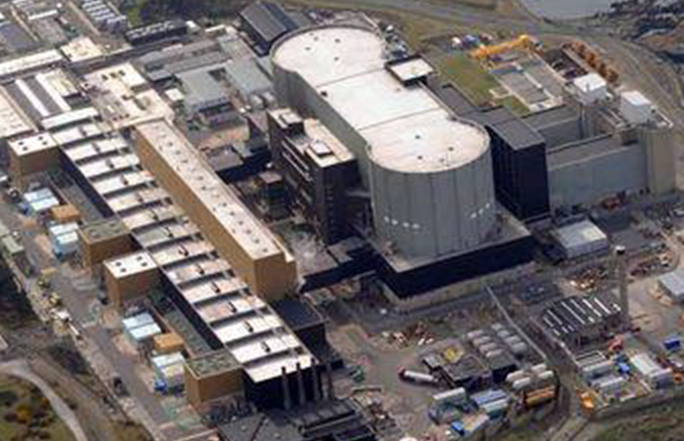
\includegraphics[width=\linewidth]{Chapter5/Figs/Raster/wylfaArielView.png}
  \captionsetup{width=.9\linewidth}
  \caption{}
  \label{subFig:wylfaArielView}
\end{subfigure}
\caption{(a) Google Maps aerial photography image, displaying the Wylfa reactor site as well as the approximate detector position. The detector is in the middle of many site buildings occluding the incident cosmic rays. Key buildings shown are the reactor building, the turbine hall and the steam pipe connections between the two \cite{GoogleMapsWylfaLink}. (b) An aerial view of the Wylfa power station the main reactor building is the shape of a "dog bone" the detector was placed in-between the turbine hall and reactor building. Edited from \cite{wylfaDronePictureLink}.}
\label{fig:DetectorPosition_TopDownAndAriel}
\end{figure}

% \begin{figure}[!h]
%  \centering
%  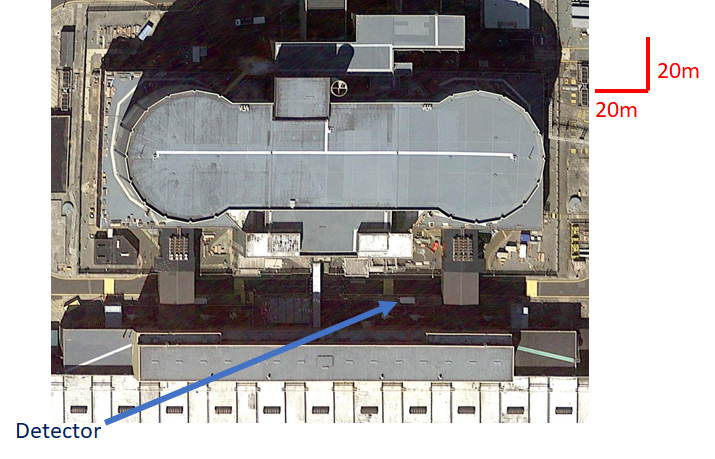
\includegraphics[width=0.75\linewidth]{Chapter5/Figs/wylfaRasterNew/DetectorPositionTopDown.png}
%  \captionof{figure}{Google Maps aerial photography image, displaying the Wylfa reactor site as well as the approximate detector position. The detector is in the middle of many site buildings occluding the incident cosmic rays. Key buildings shown are the reactor building, the turbine hall and the steam pipe connections between the two \cite{GoogleMapsWylfaLink}.} 
%  \label{fig:DetectorPositionTopDown}
% \end{figure}

% \begin{figure}[!h]
%  \centering
%  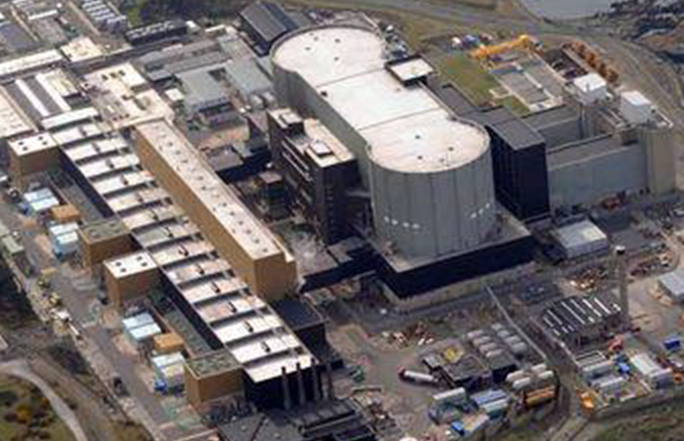
\includegraphics[width=0.6\linewidth]{Chapter5/Figs/Raster/wylfaArielView.png}
%  \captionof{figure}{An aerial view of the Wylfa power station the main reactor building is the shape of a "dog bone" the detector was placed in-between the turbine hall and reactor building. Edited from \cite{wylfaDronePictureLink}.} 
%  \label{fig:wylfaAir}
% \end{figure}

In addition, the composition of these buildings needs to be considered as well. The reactor building structure is seen in figure \ref{fig:wylfaReactorRoughStructure} with the top half of the structure being air wrapped in a concrete skin and the bottom half being thick concrete shielding. As a result, any cosmic $\mu$ events that traverse through the top of the section will have a much greater chance to penetrate than those traversing at lower angles of $\theta$. This will have two important impacts on the data set firstly it will mean that the tops of the buildings will be ``blurred'' to some extent as the amount of material will be initially low. Secondly, it will mean that the transmission value will decrease with the $\theta$ value. This decrease will be especially pronounced where the reactor core and reactor shielding would be located. 

\begin{figure}[!h]
 \centering
 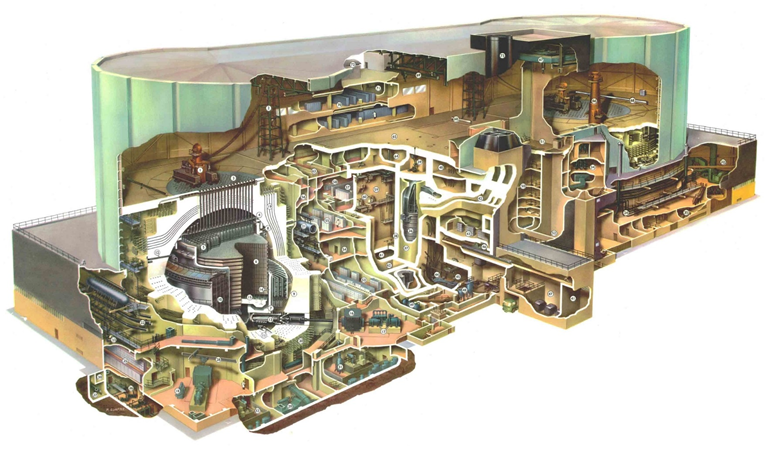
\includegraphics[width=0.6\linewidth]{Chapter5/Figs/wylfaRasterNew/wylfaReactorRoughStructure.png}
 \captionof{figure}{A cutaway diagram from \cite{neiMag_1965}. Shows the internal structure of the Wylfa reactor buildings from the back. The bottom half of the reactor buildings have thick concrete walls whilst the upper section is mostly storage. As this is a qualitative illustration of the building for public communication, the exact details, locations of features and proportions may not match the exact physical structure.} 
 \label{fig:wylfaReactorRoughStructure}
\end{figure}

\section{Reactor Shadow: Methodology} \label{sec:ReactorShadowMethodology}
In order to determine any shadows present at the reactor site the detector position relative to any buildings that block cosmic $\mu$ needs to be determined. Figure \ref{subFig:DetectorPositionTopDown} already shows the detector position as observed by Google Earth. In figure \ref{subFig:wylfaTraceStep1}, the buildings have had simple shapes overlaid on top of them with a corresponding key to highlight the buildings of interest. In figure \ref{subFig:wylfaTraceStep2} these shapes are then offset to account for the building heights relative to the detector and the angle of the aerial photograph. The most obvious anchor points in figure \ref{fig:wylfaTraceSteps1-2} being the top left of the main reactor building and top left of the turbine hall denoted with a light blue $\times$. The turbine hall offset is slightly different. Finally, the connecting lines and the background aerial photo from figure \ref{subFig:wylfaTraceStep2} are removed to produce figure \ref{fig:wylfaTraceStep4}, producing the final clean trace. In figures \ref{subFig:wylfaTraceStep1}  -- \ref{fig:wylfaTraceStep4} the size of the reactor core area is roughly inferred from private communications to be a cylinder with a diameter of $\sim$ 25\,m including both the reactor core and reactor core shielding. This inference is later corroborated with measurements from the Wylfa data set. 


\begin{figure}[!h]
\centering
\begin{subfigure}{.5\textwidth}
  \centering
  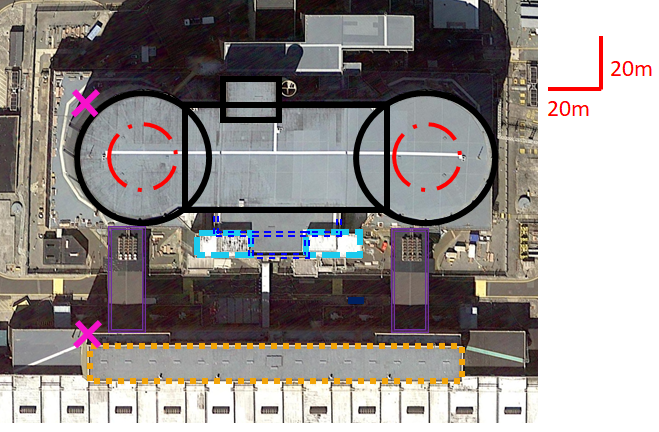
\includegraphics[width=\linewidth]{Chapter6/Figs/wylfaTraceStep1NoLeg.png}
  \captionsetup{width=.9\linewidth}
  \caption{}
  \label{subFig:wylfaTraceStep1}
\end{subfigure}%
\begin{subfigure}{.5\textwidth}
  \centering
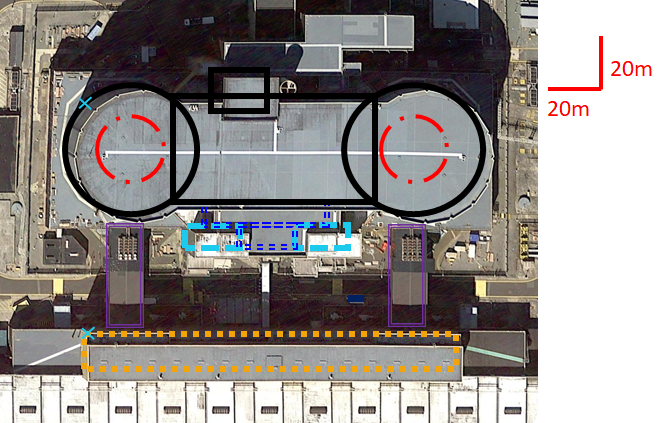
\includegraphics[width=\linewidth]{Chapter6/Figs/wylfaTraceStep2NoLeg.png}
  \captionsetup{width=.9\linewidth}
  \caption{}
  \label{subFig:wylfaTraceStep2}
\end{subfigure}
\caption{(a) a basic trace on top of figure \ref{subFig:DetectorPositionTopDown}. Basic shapes are overlaid on top of the buildings at Wylfa. In (b) the trace is adjusted to take the overhead camera's position into account by taking the base of the buildings and moving the trace towards the base of the buildings. The key is shown in figure \ref{fig:wylfaTraceStep4}. The cyan $\times$s show the anchor points used to account for the camera's position.}
\label{fig:wylfaTraceSteps1-2}
\end{figure}

% \begin{figure}[!h]
%  \centering
%  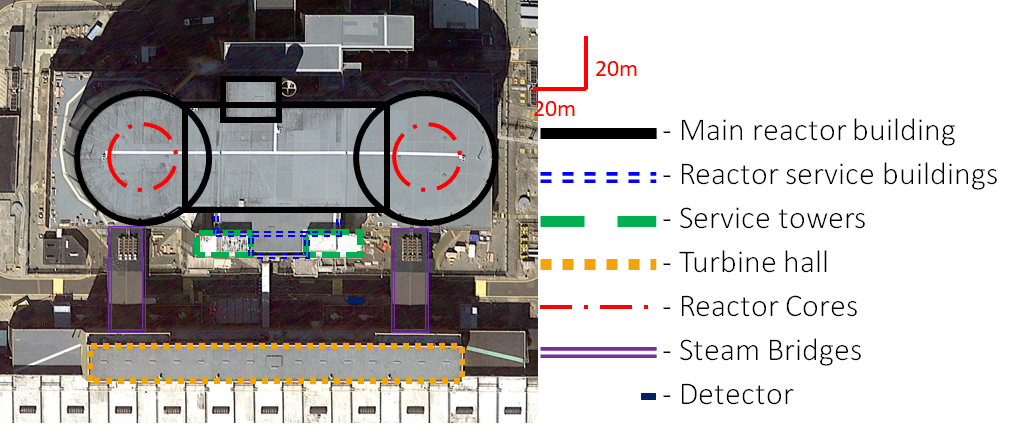
\includegraphics[width=\linewidth]{Chapter5/Figs/wylfaRasterNew/wylfaTraceStep1.png}
%  \captionof{figure}{A basic trace on top of figure \ref{subFig:DetectorPositionTopDown}. Basic shapes are overlaid on top of the buildings at Wylfa.} 
%  \label{fig:wylfaTraceStep1}
% \end{figure}

% \begin{figure}[!h]
%  \centering
%  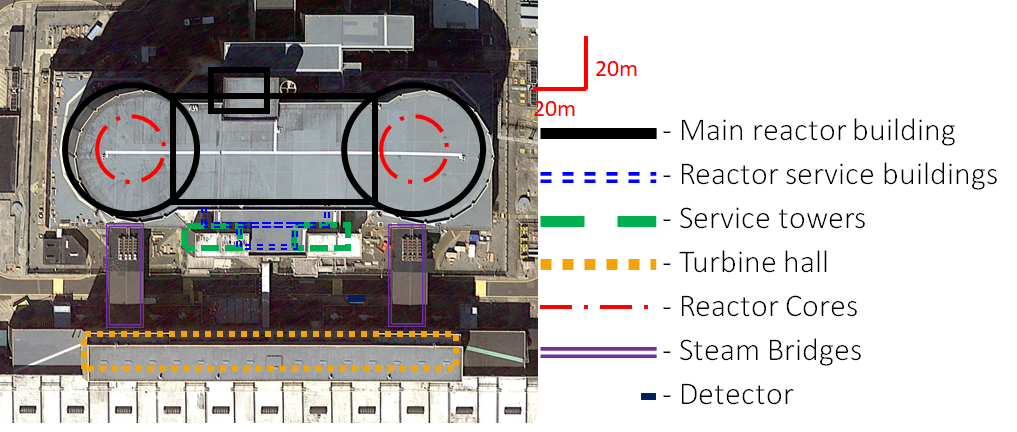
\includegraphics[width=\linewidth]{Chapter5/Figs/wylfaRasterNew/wylfaTraceStep2.png}
%  \captionof{figure}{Figure \ref{fig:wylfaTraceStep1} with the trace adjusted to take the overhead camera's position into account. By taking the base of the buildings and moving the trace towards the base of the buildings.} 
%  \label{fig:wylfaTraceStep2}
% \end{figure}

% \begin{figure}[!h]
%  \centering
%  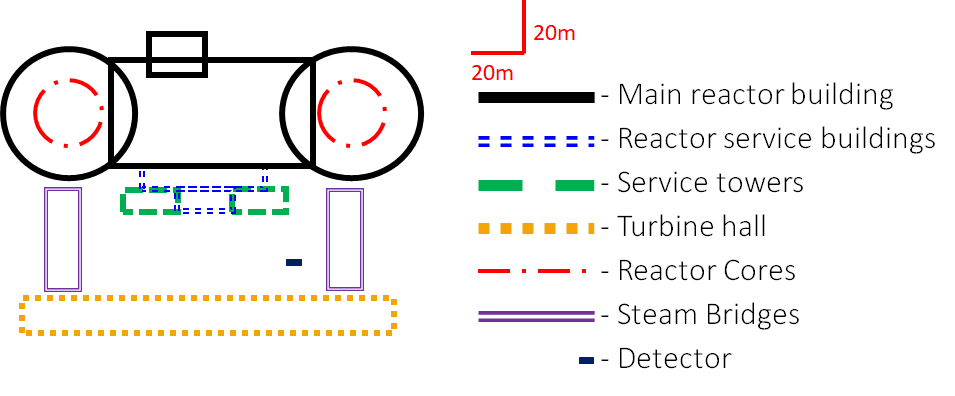
\includegraphics[width=\linewidth]{Chapter5/Figs/wylfaRasterNew/wylfaTraceStep3.png}
%  \captionof{figure}{.} 
%  \label{fig:}
% \end{figure}

\begin{figure}[!h]
 \centering
 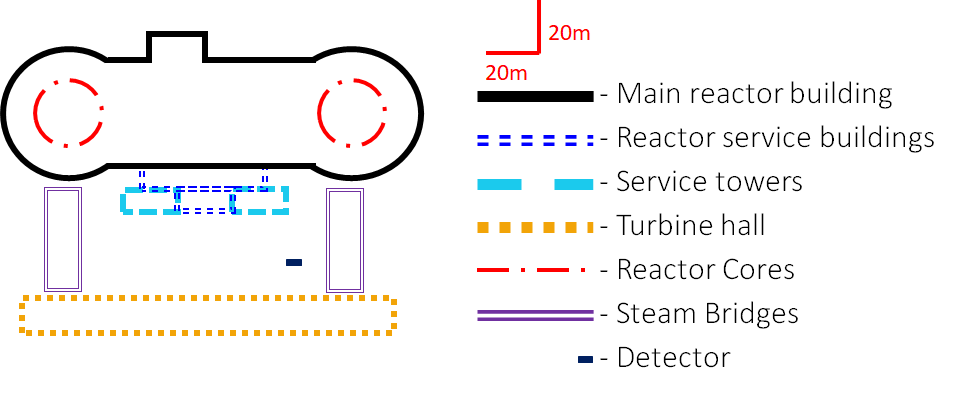
\includegraphics[width=\linewidth]{Chapter5/Figs/wylfaRasterNew/wylfaTraceStep4.png}
 \captionof{figure}{Figure \ref{subFig:wylfaTraceStep2} with the overlapping lines and aerial photography from Google Earth removed to produce the final trace.}
 \label{fig:wylfaTraceStep4}
\end{figure}

Now that figure \ref{fig:wylfaTraceStep4} has been produced and the features of interest have been identified the cosmic $\mu$ data needs to be analysed. The logic for the track fitter is outlined in section \ref{sec:SimulationOfCosmics}, using that tracker the Wylfa data can be fitted. An example even can be seen in figure \ref{fig:3000ExampleEventWithKey}. In figure \ref{fig:3000ExampleEventWithKey} there are many noise events that can potentially cause the track fitter to struggle. The tracker however has been custom-built around the data set to help prevent any minimisation issues. There are also 3 columns of un-instrumented channels on side A which figure \ref{fig:3000ExampleEventWithKey} shows in grey. These un-instrumented channels inform the fidicual boundaries as well, which figure \ref{fig:3000ExampleEventWithKey} shows in light blue. The number of columns on side A and Side B must be the same otherwise any shadow that the detector will analyse will become distorted in one direction more than the other. Also in figure \ref{fig:3000ExampleEventWithKey} there are a number of dead channels that also have to be carefully considered when assessing tracker performance. By looking at the tracker reconstructed hits on aggregate in figure \ref{fig:wylfaSideABHits} there does not appear to be any bias in the Wylfa data set. In figure \ref{fig:wylfaSideABHits} the are dead channels and channels that fire rarely don't have halos of low statistics around them suggesting the tracker is successfully representing the distribution. The only issue is a noisy channel in \ref{subFig:wylfaSideBHits} but as the areas around the channel have statistics comparable to their neighbours it's reasonable to assume this is an issue with the channel rather than the fitter. 

\begin{figure}[!h]
 \centering
 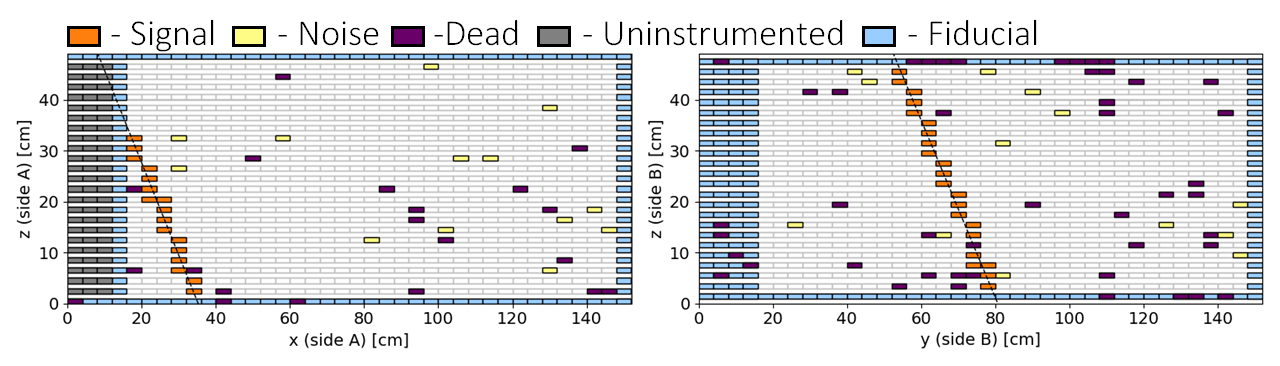
\includegraphics[width=\linewidth]{Chapter6/Figs/newExampleEventWylfa.png}
 \captionof{figure}{An example event from the Wylfa data set with a corresponding key showing how the colour coding relates to the channels. The dashed line represents the fit.} 
 \label{fig:3000ExampleEventWithKey}
\end{figure}

\begin{figure}[!h]
\centering
\begin{subfigure}{.5\textwidth}
  \centering
  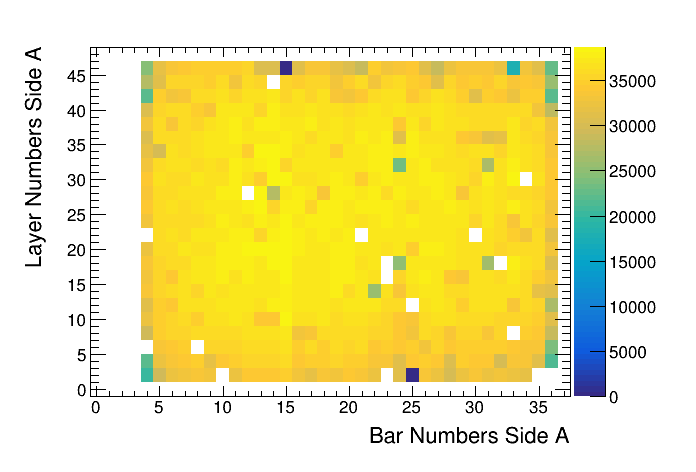
\includegraphics[width=\linewidth]{Chapter5/Figs/wylfaRasterNew/wylfaSideAHits.png}
  \captionsetup{width=.9\linewidth}
  \caption{}
  \label{subFig:wylfaSideAHits}
\end{subfigure}%
\begin{subfigure}{.5\textwidth}
  \centering
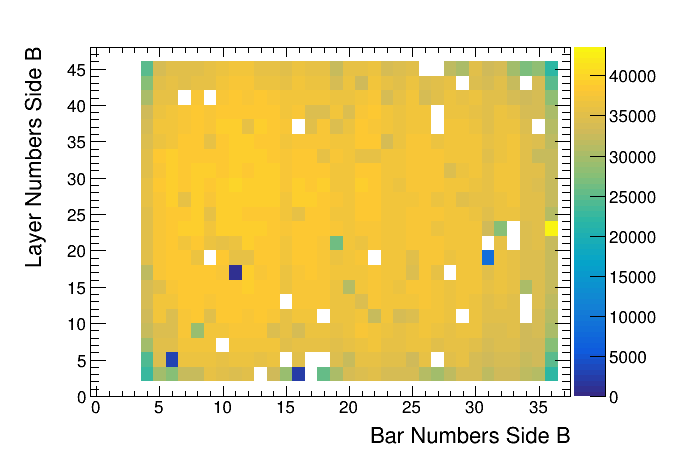
\includegraphics[width=\linewidth]{Chapter5/Figs/wylfaRasterNew/wylfaSideBHits.png}
  \captionsetup{width=.9\linewidth}
  \caption{}
  \label{subFig:wylfaSideBHits}
\end{subfigure}
\caption{Bars hit for sides A and B cosmic $\mu$ reconstructed tracks for the Wylfa data set. The results are mostly even except for a few dead or almost dead channels and one noisy channel on side B. Suggesting the tracker has minimal biasing. Side A is shown in (a). Side B is Shown in (b)}
\label{fig:wylfaSideABHits}
\end{figure}

Once the fitter's potential bias has been addressed the $\phi$ and $\theta$ values can be analysed. Due to the high energy and highly penetrating nature of cosmic $\mu$ \cite{Olive_2014} the reactor buildings may not be dense enough to stop all incoming cosmic $\mu$, and deflection is a likely possibility. As a result, the shadows can only be seen with high statistics. However, the detector took cosmic $\mu$ data in accidental coincidence at the Wylfa site and this greatly limited the amount of data that could be gathered to $\sim$ 3 $\times$ 10$^6$ cosmic $\mu$ events. According to the CRY library, \cite{ieee_cry_2007} 162000 $\mu^-$ and 174000 $\mu^+$ are produced in 2820\,s for 1 m\,$^2$. The Rmon's top surface area is 1.52\,m $\times$ 1.52\,m = 2.31\,m$^2$ resulting in $\sim$ 275 $\mu$ s$^{-1}$. Therefore, a data set of 3 $\times$ 10$^6$ cosmic $\mu$ events corresponds to $\sim$ 3 hours of live time. With a rate of 275 $\mu$ s$^{-1}$ the maximum time a fit should be allowed to take is 3600 microseconds for online track fitting which figure \ref{subFig:wylfaTrackerTime} shows is the case for almost all events. Figure \ref{fig:wylfaTrackerTimeAndLog} shows that only a very small fraction of events don't fit within the time limit of 3600 microseconds so a time selection criteria will be required for online track fitting. Whilst online track fitting was not required, it is useful to know that the same tracker logic can be applied for both online calibration and full cosmic $\mu$ tomography by only adding a time selection cut. 

\begin{figure}[!h]
\centering
\begin{subfigure}{.5\textwidth}
  \centering
  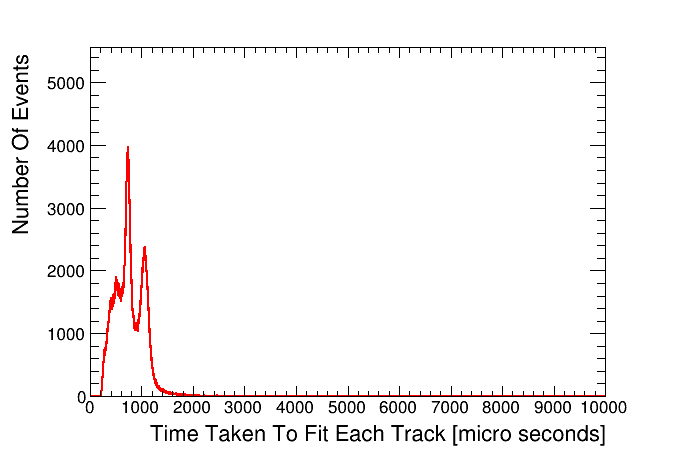
\includegraphics[width=\linewidth]{Chapter5/Figs/Raster/wylfaTrackerTime.png}
  \captionsetup{width=.9\linewidth}
  \caption{}
  \label{subFig:wylfaTrackerTime}
\end{subfigure}%
\begin{subfigure}{.5\textwidth}
  \centering
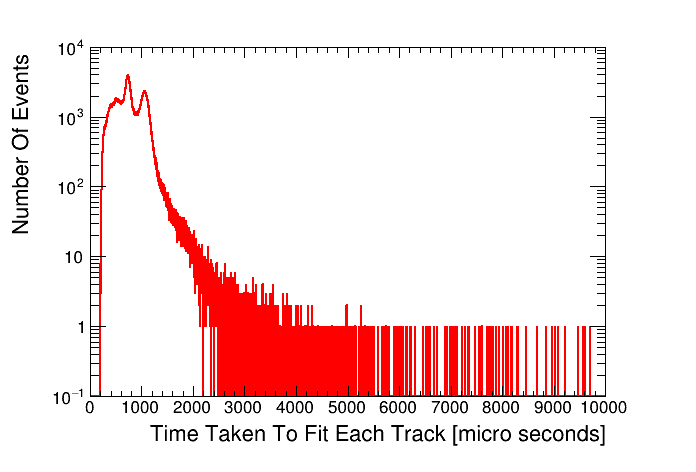
\includegraphics[width=\linewidth]{Chapter5/Figs/Raster/wylfaTrackerTimeLog.png}
  \captionsetup{width=.9\linewidth}
  \caption{}
  \label{subFig:wylfaTrackerTimeLog}
\end{subfigure}
\caption{(a) The time taken for each fit for the Wylfa data set. Assuming a rate of $\sim$ 275 cosmic $\mu$ s$^{-1}$ then the maximum time allowed would be 3600 microseconds. Almost all cosmic candidate events fit within this time. (b) Figure \ref{subFig:wylfaTrackerTime} but with the y axis taken as a log some events exceed 3600 microseconds to fit so a maximum time selection criterion is needed for those events.}
\label{fig:wylfaTrackerTimeAndLog}
\end{figure}

The reconstructed $\phi$ and $\theta$ distribution from the Wylfa data set can be seen in figure \ref{fig:pVsTWylfaReversed} but the shadows don't seem as clear as one would have expected from such large and dense buildings. In figure \ref{fig:pVsTWylfaReversed} the bin migration is so significant even though the shadows extend up to 60$^o$ in $\theta$ they are effectively masked. But the bin migration does become less pronounced as $\theta$ decreases, As the chance of either side of the detector having a vertical track is greatly reduced (see section \ref{sec:SimulationOfCosmics}). However, this poses a problem as the statistics also decrease with $\theta$ as seen in figure \ref{fig:pVsTWylfaReversed}. So by taking the 2D x projection of figure \ref{fig:pVsTWylfaReversed} from 0$^\circ$ -- 37.5$^\circ$ in $\theta$ it is possible to ignore most of the bin migration whilst also having suitable statistics to observe the widths of the turbine hall and reactor building which is done in figure \ref{fig:LinearHist_theta_0-37.5_Deg}. Figure \ref{fig:LinearHist_theta_0-37.5_Deg} is then and shown it via a circular histogram and overlaid on top of the Wylfa trace (figure \ref{fig:wylfaTraceStep4}) producing figure \ref{fig:wylfaCircular0-37.5Deg_Overlay}. 

\begin{figure}[!h]
\centering
\begin{minipage}{.45\textwidth}
  \centering
  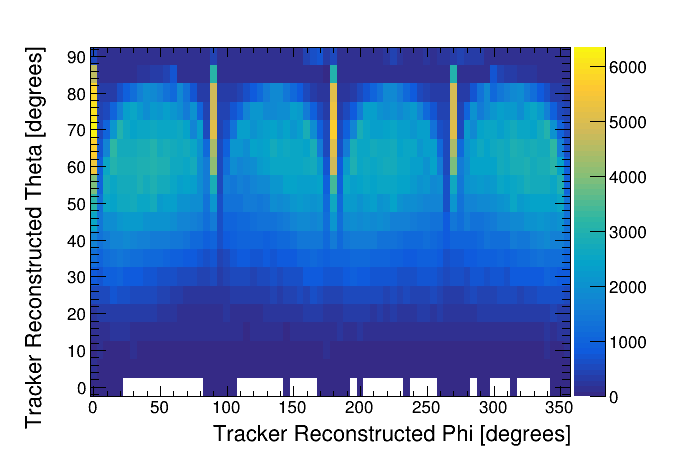
\includegraphics[width=\linewidth]{Chapter5/Figs/Raster/pVsTWylfaReversed.png}
  \captionof{figure}{The cosmic $\mu$ distribution from Rmon deployment at Wylfa the shadows extend from $\theta$ = 0$^\circ$ -- $\theta$ = 60$^\circ$. Bin migration causes signifficant warping.}
  \label{fig:pVsTWylfaReversed}
\end{minipage}%
\qquad
\begin{minipage}{.45\textwidth}
  \centering
  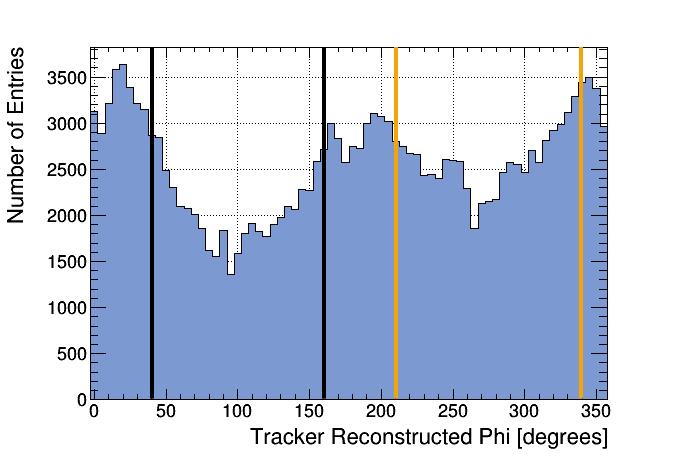
\includegraphics[width=\linewidth]{Chapter5/Figs/wylfaRasterNew/LinearHist_theta_0-37.5_Deg.png}
  \captionof{figure}{Linear histogram showing a 2d projection of figure \ref{fig:pVsTWylfaReversed} from $\theta$ = 0$^\circ$ -- $\theta$ = 37.5$^\circ$ this range was chosen to avoid as much bin migration as possible whilst having as high statistics as possible. The main reactor shadow is highlighted by black lines the turbine hall is highlighted by orange lines.}
  \label{fig:LinearHist_theta_0-37.5_Deg}
\end{minipage}
\end{figure}

 \begin{figure}[!h]
 \centering
 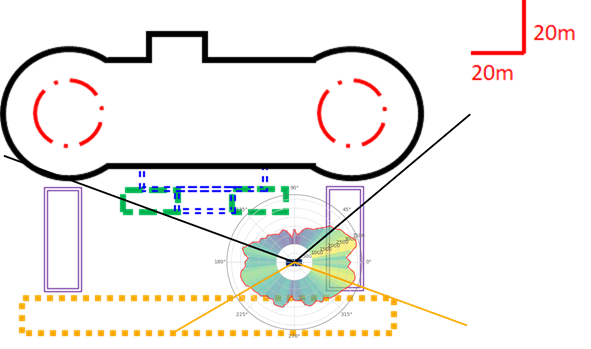
\includegraphics[width=0.7\linewidth]{Chapter5/Figs/wylfaRasterNew/wylfaCircular0-37.5Deg_Overlay.png}
 \captionof{figure}{Figure \ref{fig:wylfaTraceStep4} overlaid with the circular histogram from figure \ref{fig:LinearHist_theta_0-37.5_Deg} to show how the borders line up with the Wylfa trace.} 
 \label{fig:wylfaCircular0-37.5Deg_Overlay}
\end{figure}

Figure \ref{fig:wylfaCircular0-37.5Deg_Overlay} also shows the limitation of this method. Whilst there are several buildings that should block incident cosmic $\mu$ only the largest building (the main reactor building) and the closest building (the turbine hall) are visible. In addition, the far edge of the turbine hall is not clear in figure \ref{fig:wylfaCircular0-37.5Deg_Overlay}, even though it should be. This is due to the composition of the turbine hall being corrugated steel, thus blocking fewer cosmic $\mu$. The results from figures \ref{fig:pVsTWylfaReversed} -- \ref{fig:wylfaCircular0-37.5Deg_Overlay} match closely to what we expected to see as figure \ref{fig:sideBySideComparisonTopDownCirc} shows. 

 \begin{figure}[!h]
 \centering
 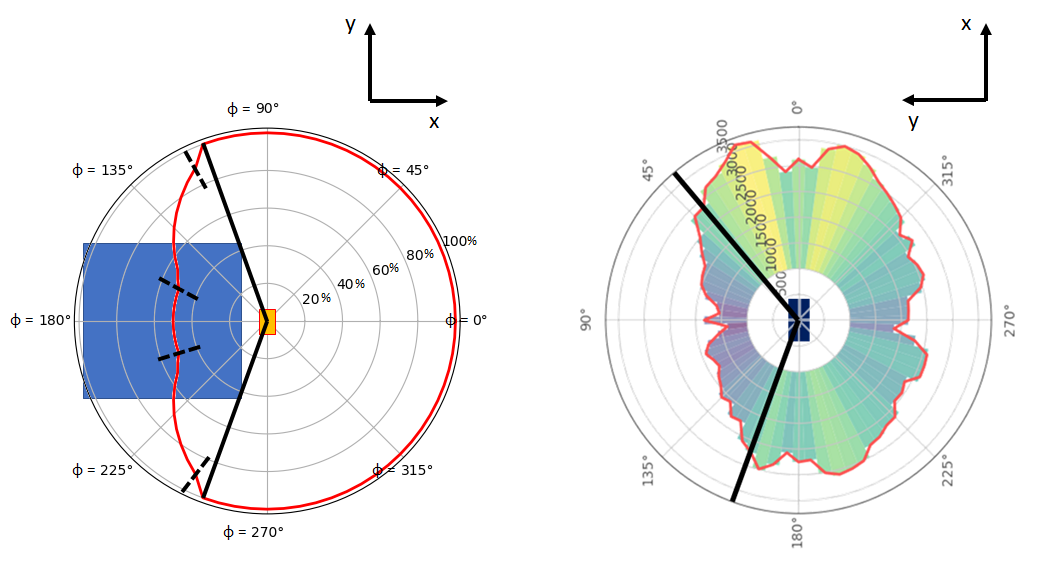
\includegraphics[width=\linewidth]{Chapter5/Figs/wylfaRasterNew/sideBySideComparisonTopDownCirc.png}
 \captionof{figure}{How the circular Wylfa histogram compares to a basic expectation the large tails are visible in both producing a similar shape.}
 \label{fig:sideBySideComparisonTopDownCirc}
\end{figure}

A way to solve the issue of bin migration was highlighted in section \ref{sec:murayTomographyAndTransmissionMethod} which is to use the transmission method the MU-RAY collaboration have done in figure \ref{fig:mtVesuviusMuRayTransmission} \cite{Ambrosino_2014}. The transmission method is where the data with the cosmic $\mu$ blockage has a ratio taken with a control data set which has minimal to no $\mu$ blockage. In order for this to work, another data set that reconstructs the whole hemisphere in $\phi$ and $\theta$ is required. It might be possible to use simulated cosmic data to achieve this result however the atmospheric scattering isn't taken into account properly (As will be shown in section \ref{sec:usingSimulatedDataAsControlData}). The best approach would be to use measured data in the same location after the demolition of the Wylfa buildings, but as that will take decades this is infeasible. Instead, measured data was taken at Liverpool from 2016 -- 2018 which produced figure \ref{fig:pVsTLiverpoolReversed}. There are some shadows in the Liverpool data specifically from the accelerator hall at low angles of $\theta$ from 0$^\circ$ -- 17.5$^\circ$ which is shown in figure \ref{fig:liverpoolShadows}. However, once those ranges are removed from the data set it serves as a useful control as there is minimal cosmic $\mu$ sky blockage. When checking for any potential bias in the Liverpool data set none is visible in either side as shown in figure \ref{fig:liverpoolSideABHits}. 

\begin{figure}[!h]
\centering
\begin{minipage}{.45\textwidth}
  \centering
  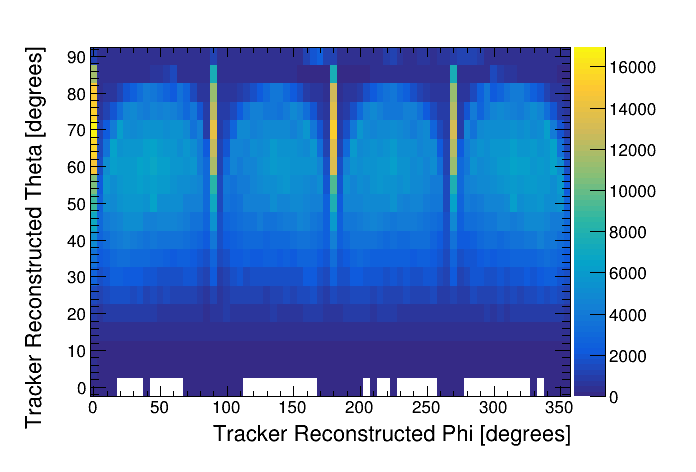
\includegraphics[width=\linewidth]{Chapter5/Figs/Raster/pVsTLiverpoolReversed.png}
  \captionof{figure}{The cosmic $\mu$ distribution from the Rmon deployment at Liverpool. There are some faint shadows below 17.5$^\circ$ but otherwise, the data has no major cosmic $\mu$ sky blockage.} 
  \label{fig:pVsTLiverpoolReversed}
\end{minipage}%
\qquad
\begin{minipage}{.45\textwidth}
  \centering
  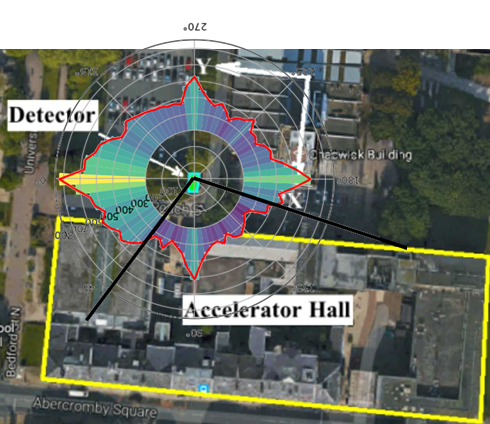
\includegraphics[width=\linewidth]{Chapter5/Figs/Raster/liverpoolShadows.png}
  \captionof{figure}{The shadows in the Liverpool data below $\theta$ 17.5$^\circ$. The accelerator Hall causes significant cosmic $\mu$ blockage.}
  \label{fig:liverpoolShadows}
\end{minipage}
\end{figure}

\begin{figure}[!h]
\centering
\begin{subfigure}{.5\textwidth}
  \centering
  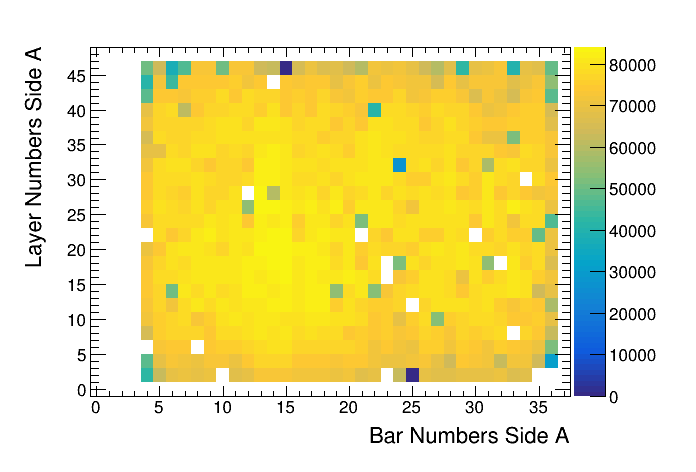
\includegraphics[width=\linewidth]{Chapter5/Figs/wylfaRasterNew/liverpoolSideAHits.png}
  \captionsetup{width=.9\linewidth}
  \caption{}
  \label{subFig:liverpoolSideAHits}
\end{subfigure}%
\begin{subfigure}{.5\textwidth}
  \centering
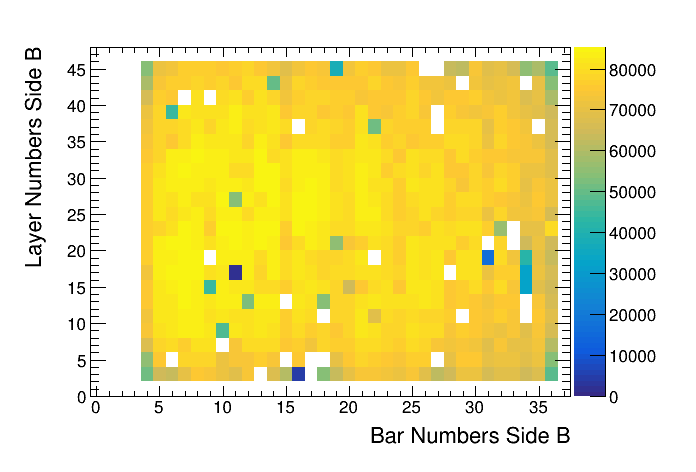
\includegraphics[width=\linewidth]{Chapter5/Figs/wylfaRasterNew/liverpoolSideBHits.png}
  \captionsetup{width=.9\linewidth}
  \caption{}
  \label{subFig:liverpoolSideBHits}
\end{subfigure}
\caption{Bars hit for sides A and B cosmic $\mu$ reconstructed tracks for the Liverpool data set. The results are mostly even except for a few dead or almost dead channels. Suggesting the tracker has minimal biasing. Side A is shown in (a). Side B is shown in (b).}
\label{fig:liverpoolSideABHits}
\end{figure}

When taking the Wylfa data (figure \ref{fig:pVsTWylfaReversed}) and dividing it by the Liverpool data (figure \ref{fig:pVsTLiverpoolReversed}) and normalising the Liverpool data set to the Wylfa data set and removing the values below 17.5$^\circ$ in $\theta$ (thus making the Liverpool data suitable for control purposes) a map of Wylfa shadows with minimal detector effects is produced (figure \ref{fig:measuredTrackerReconNoLines}). The shadows are now clearly visible in both $\phi$ and $\theta$ with the main reactor buildings centring around 90$^\circ$ in $\phi$ and the turbine hall centring around 270$^\circ$ in $\phi$. There are several interesting features seen in figure \ref{fig:measuredTrackerReconNoLines} the top of the turbine hall seen between $\sim$ 240$^\circ$ -- 330$^\circ$ in $\phi$ is not well resolved. This is because the turbine hall is made from corrugated steel and so blocks fewer cosmic $\mu$. Therefore, a significant portion of the building has to be traversed before the top is visible. But the area from 0$^\circ$ -- 180$^\circ$ in $\phi$ is of particular interest as this area contains the main reactor building but also several others. As a result of multiple buildings blocking the path of incident cosmic $\mu$ between the detector and reactor building the shadow, patterns are much more complex than one would expect. In addition, there appears to be an area of high density between 60$^\circ$ -- 80$^\circ$ in $\phi$, 20$^\circ$ -- 25$^\circ$ in $\theta$ which could be the reactor core. In order to determine which components of the shadow are caused by which buildings a simulation is required where each reactor building can be simulated separately.

\begin{figure}[!h]
 \centering
 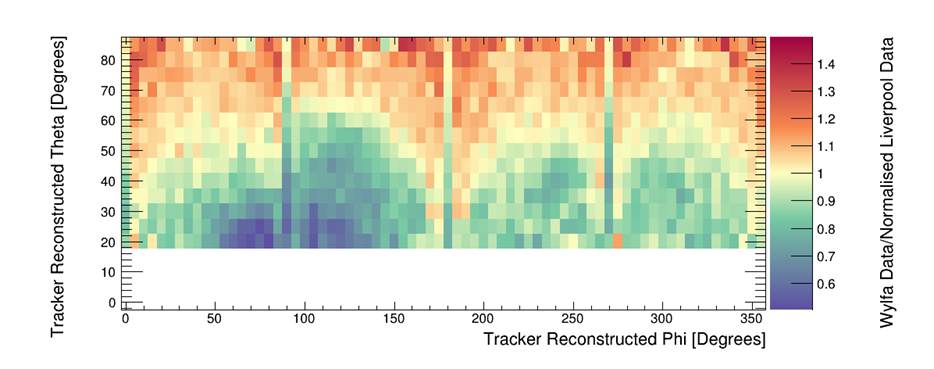
\includegraphics[width=\linewidth]{Chapter5/Figs/wylfaRasterNew/measuredTrackerReconNoLines.png}
 \captionof{figure}{The measured building shadows taking the ratio of the Wylfa data set (figure \ref{fig:pVsTWylfaReversed}) and the Liverpool data set (figure \ref{fig:pVsTLiverpoolReversed}) with the Liverpool data acting as a control data set assuming minimal shadows are present in the Liverpool data above 17.5$^\circ$ in $\theta$ as there are no dense buildings above 17.5$^\circ$ in $\theta$ at Liverpool.} 
 \label{fig:measuredTrackerReconNoLines}
\end{figure}

The simulation previously mentioned in chapter \ref{chp:GEANT4Simulation} has the detector as the centre of the simulation world in the $x$ and $y$ and put the detector on the floor at  $z = 0 $. As such all of the reactor buildings need to be positioned relative to the detector and also placed at $z = 0$. The Wylfa trace seen in figure \ref{fig:wylfaTraceStep4} can be approximated by having simple shapes placed on top of the trace as seen in figure \ref{fig:simulatedPositions}. Figure \ref{fig:simulatedPositions} also clearly labels each major building box, the positions for each box and in x and y and the widths and depths are approximated from this figure and are seen in table \ref{tab:simulatedBuildingPositions}. Finally, the heights have to be approximated: this is difficult due to the distortion tops of buildings are subject to as part of projecting a comic hemisphere distribution onto a cuboid. In addition, distance, height, building shape and construction are all combined into a single measurement. This is the main reason the building widths are intuited from Google Earth rather than from measured data. Sadly, no information pertaining to heights has been preserved, it is tempting to use the measurements of $\theta$ to produce reconstructions of the heights via equation \ref{equ:tanHeightEquation} with the lengths provided by Google Earth. But this approach has two key assumptions: 1. perfectly solid uniform buildings 2. minimal scattering of cosmic $\mu$. Assumption 1 is known to be inaccurate from figure \ref{fig:wylfaReactorRoughStructure}. Assumption 2 is naive considering the high Z values and densities used in the construction of the reactor buildings. As a result, it is best to use the estimates provided by equation \ref{equ:tanHeightEquation} and then iterate over different heights in the simulation to roughly match the shadow shapes seen in figure \ref{fig:measuredTrackerReconNoLines}. The approximate heights and z positions are also shown in table \ref{tab:simulatedBuildingPositions}. Ideally, the heights in the simulation would be resolved by going on-site and taking detailed measurements. Due to the decommissioning currently taking place at the Wylfa site, this is not possible. Appendix \ref{appenC:ReactorBuildingEdges} contains the remaining building boxes simulated, the boxes which are used to emulate the distinctive ``dog bone'' shape of the main reactor building at Wylfa.

\begin{equation}
H = \frac{L}{\tan{\theta}}
\label{equ:tanHeightEquation}
\end{equation}

 \begin{figure}[!h]
 \centering
 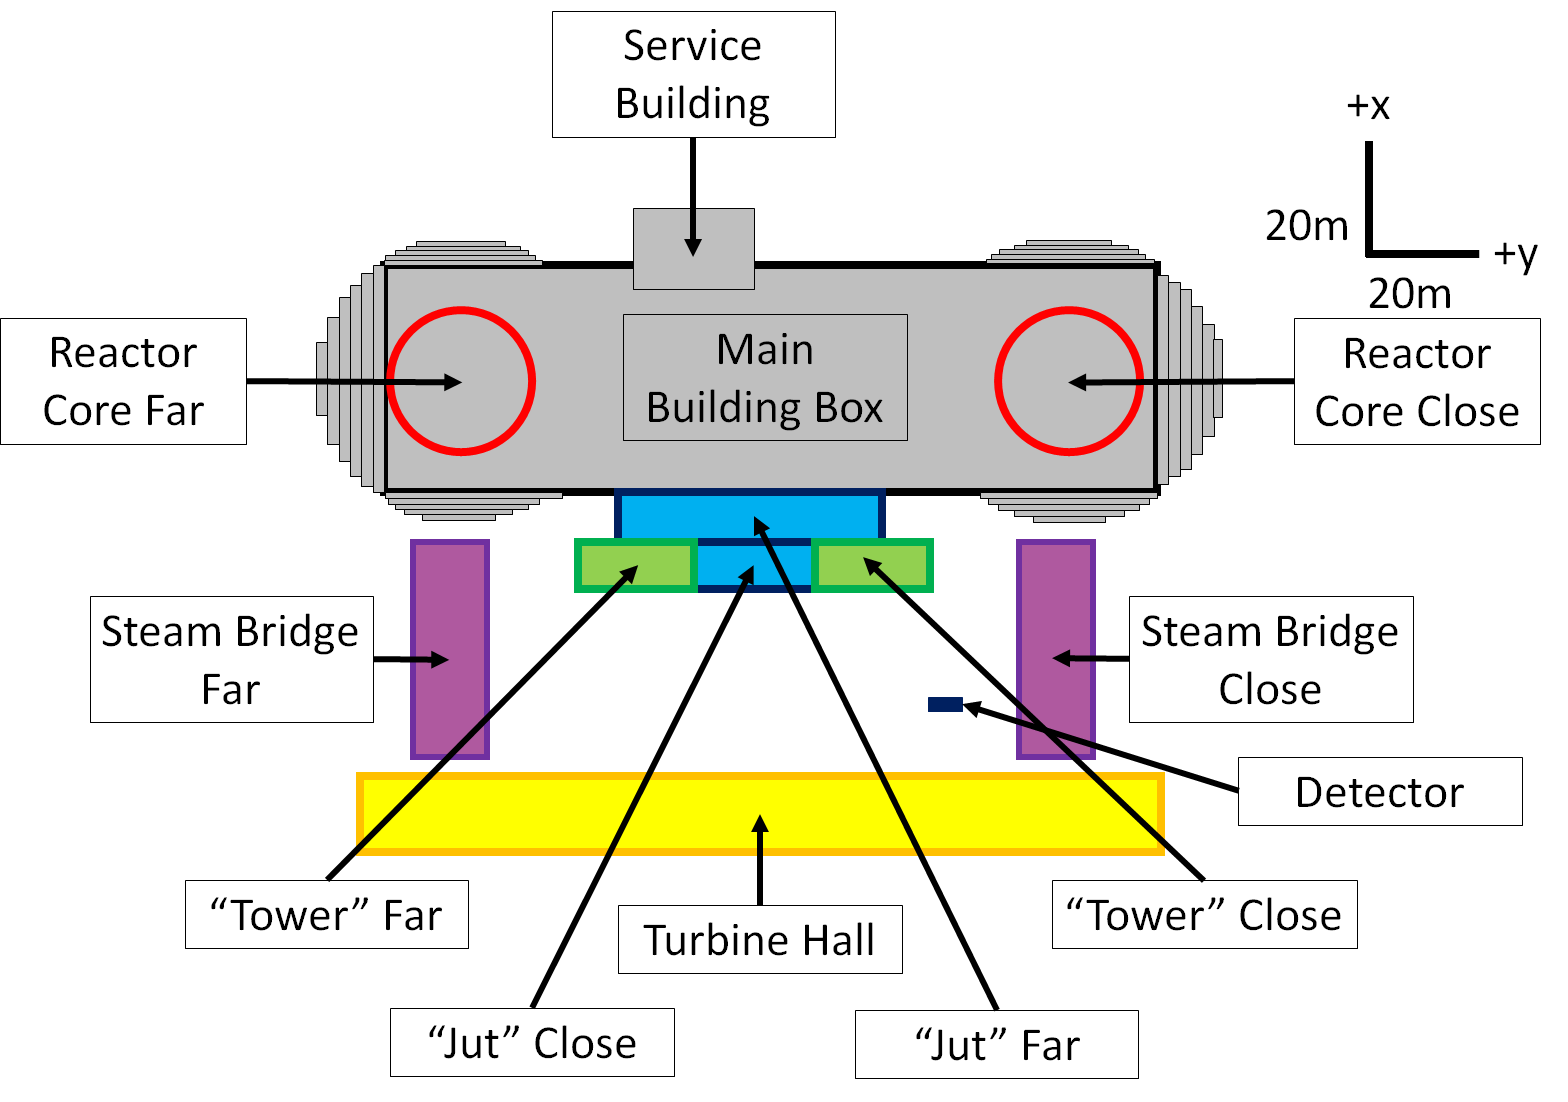
\includegraphics[width=0.7\linewidth]{Chapter6/Figs/Raster/simulatedAnotatedBuildings.png}
 \captionof{figure}{The Wylfa trace (figure \ref{fig:wylfaTraceStep4}) with boxes overlaid to recreate the buildings of interest and circles to represent the reactor cores. The scale from the Wylfa trace (top right) is used to give the buildings the correct positions and dimensions in GEANT4 a full list of which can be seen in \ref{tab:simulatedBuildingPositions}. The edges for the ``dog bone'' shape are shown in appendix \ref{appenC:ReactorBuildingEdges}.} 
 \label{fig:simulatedPositions}
\end{figure}

% \begin{figure}[!h]
%  \centering
%  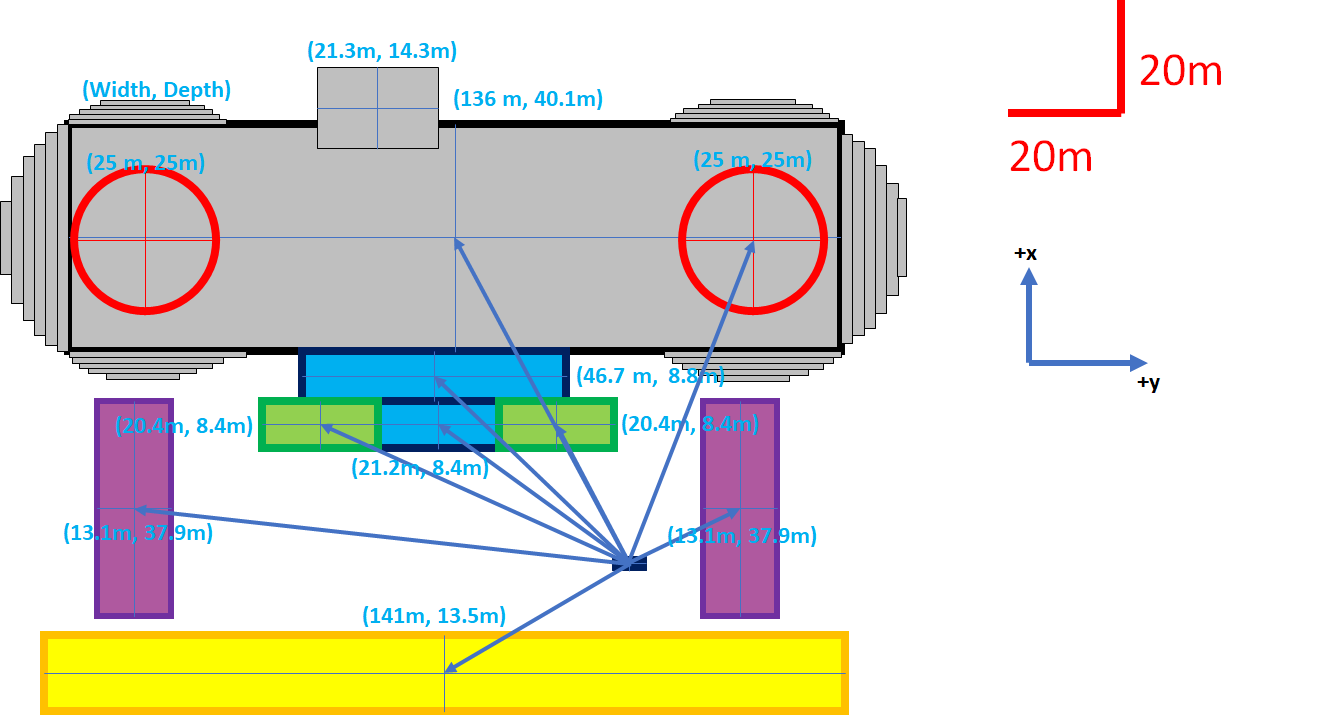
\includegraphics[width=0.8\linewidth]{Chapter5/Figs/wylfaRasterNew/simulatedWidthsDepths.png}
%  \captionof{figure}{Widths and depths from the Wylfa trace (figure \ref{fig:wylfaTraceStep4}) with their widths and depths labelled these were then put into GEANT4.} 
%  \label{fig:simulatedWidthsDepths}
% \end{figure}

% \begin{figure}[!h]
%  \centering
%  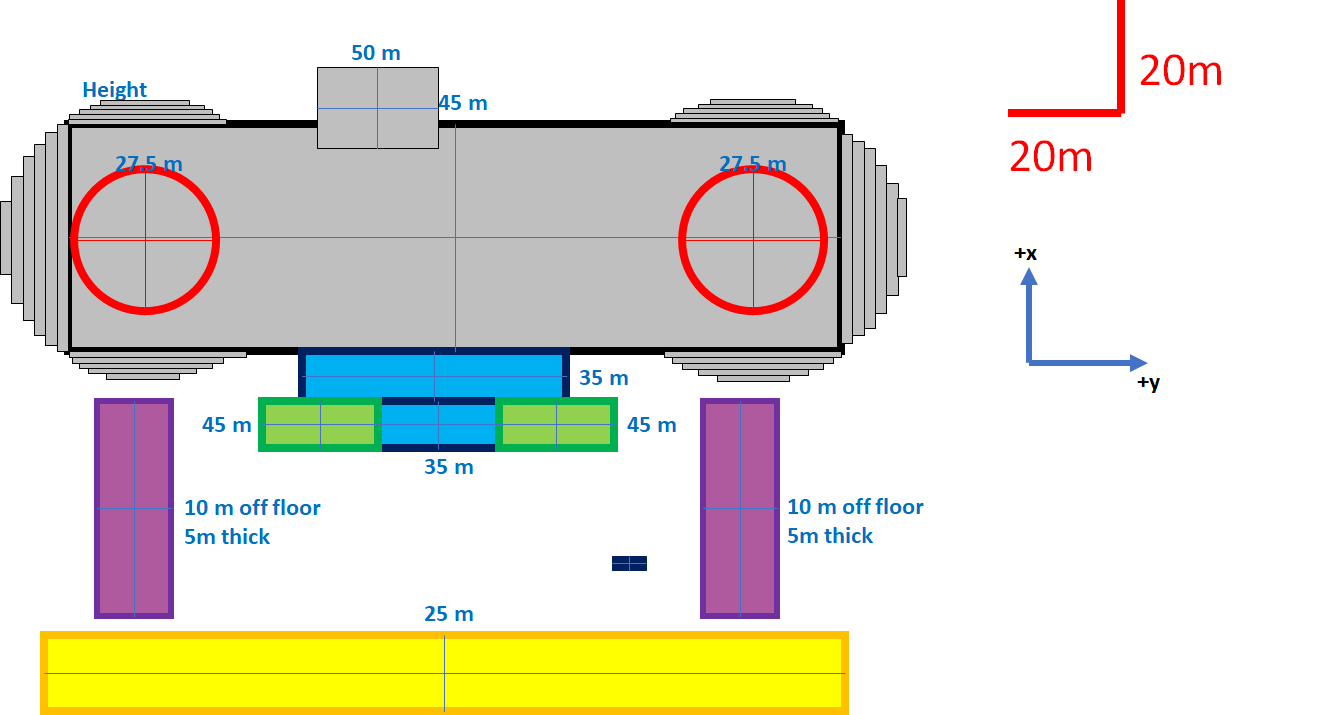
\includegraphics[width=0.8\linewidth]{Chapter5/Figs/wylfaRasterNew/simulatedHeights.png}
%  \captionof{figure}{Heights estimated from the measured data at Wylfa (figure \ref{fig:pVsTWylfaReversed}) these were then put into GEANT4.} 
%  \label{fig:simulatedHeights}
% \end{figure}

\begin{table*}[!h]
\centering
\begin{tabular}{lrrrrrrr}  
\toprule
\multicolumn{1}{c}{} & \multicolumn{3}{c}{Position} & \multicolumn{3}{c}{Dimension} \\
\cmidrule(r){2-4}
\cmidrule(r){5-7}
Building               & X\,[m] & Y\,[m] & Z\,[m] & Width\,[m] & Depth\,[m] & Height\,[m]\\
\midrule
Reactor Core Close     & 57.1   &  22.2  & 0.0     & 25.0       & 25.0       & 27.5\\
Reactor Core Far       & 57.1   & -85.3  & 0.0     & 25.0       & 25.0       & 27.5\\
Main Building Box      & 57.5   & -30.8  & 0.0     & 40.1       & 136.0      & 45.0\\
Sub Building Box       & 80.5   & -44.6  & 0.0     & 14.3       & 21.3       & 50.0\\
Service Building Close & 24.4   & -33.6  & 0.0     & 8.4        & 21.2       & 35.0\\
Service Building Far   & 33.0   & -34.4  & 0.0     & 8.8        & 46.7       & 35.0\\
Service Tower Close    & 24.4   & -12.8  & 0.0     & 8.4        & 20.4       & 45.0\\
Service Tower Far      & 24.4   & -54.5  & 0.0     & 8.4        & 20.4       & 45.0\\
Steam Bridge Close     & 9.73   &  19.7  & 10.0    & 37.9       & 13.1       & 5.0\\
Steam Bridge Far       & 9.73   & -87.7  & 10.0    & 37.9       & 13.1       & 5.0\\
Turbine Hall           & -19.2  & -32.7  & 0.0     & 13.5       & 141.0      & 25.0\\
\bottomrule  
\end{tabular}
\caption{The positions and dimensions for each of the simulated buildings in GEANT4 outlined in figure \ref{fig:simulatedPositions}, relative to the detector which is the origin.}
\label{tab:simulatedBuildingPositions}
\end{table*}

Figure \ref{fig:WylfaSimGeom_SideOn_TopDown} shows how the simulated geometry looks in  GEANT4. The side-on view can be seen in figure \ref{subFig:WylfaSimGeomSideOn} which has the heights annotated, and the top-down view can be seen in figure \ref{subFig:WylfaSimGeomTopDown} which looks similar to figure \ref{fig:simulatedPositions}. Once these dimensions have been approximated, it is possible to simulate both with and without buildings. This is done in figure \ref{fig:thetaVsPhiSimulatedWithReactor_0-100} which shows how the bin migration effects compare with the shadows. In the simulation the buildings were simulated as 100\,\% concrete, this is done so they block as many cosmic $\mu$ as possible to give accurate building outlines. Then as with the shadows at Wylfa (figure \ref{fig:measuredTrackerReconNoLines}) the ratio of the data with and without buildings is taken producing the simulated shadows with minimal detector effects (figure \ref{fig:simulatedTrackerReconNoLines}). 

\begin{figure}[!h]
\centering
\begin{subfigure}{.5\textwidth}
  \centering
  \includegraphics[width=\linewidth]{Chapter5/Figs/wylfaRasterNew/WylfaSimGeomSideOn.png}
  \captionsetup{width=.9\linewidth}
  \caption{}
  \label{subFig:WylfaSimGeomSideOn}
\end{subfigure}%
\begin{subfigure}{.5\textwidth}
  \centering
\includegraphics[width=\linewidth]{Chapter5/Figs/wylfaRasterNew/WylfaSimGeomTopDown.png}
  \captionsetup{width=.9\linewidth}
  \caption{}
  \label{subFig:WylfaSimGeomTopDown}
\end{subfigure}
\caption{The simulated geometry in GEANT4. (a) shows the side on view (y,z) with heights annotated. (b) shows the top-down perspective. Relative to the detector which is the origin.}
\label{fig:WylfaSimGeom_SideOn_TopDown}
\end{figure}

\begin{figure}[!h]
\centering
\begin{subfigure}{.5\textwidth}
  \centering
  \includegraphics[width=\linewidth]{Chapter5/Figs/wylfaRasterNew/thetaVsPhiSimulatedWithReactor0.png}
  \captionsetup{width=.9\linewidth}
  \caption{}
  \label{subFig:thetaVsPhiSimulatedWithReactor0}
\end{subfigure}%
\begin{subfigure}{.5\textwidth}
  \centering
\includegraphics[width=\linewidth]{Chapter5/Figs/wylfaRasterNew/thetaVsPhiSimulatedWithReactor100.png}
  \captionsetup{width=.9\linewidth}
  \caption{}
  \label{subFig:thetaVsPhiSimulatedWithReactor100}
\end{subfigure}
\caption{A side by side comparison of the GEANT4 simulation $\phi$ and $\theta$ distributions without reactor buildings (seen in (a)) and with reactor buildings (seen in side (b)) using a realistic $\theta$ distribution.}
\label{fig:thetaVsPhiSimulatedWithReactor_0-100}
\end{figure}

\begin{figure}[!h]
 \centering
 \includegraphics[width=\linewidth]{Chapter5/Figs/wylfaRasterNew/simulatedTrackerReconNoLines.png}
 \captionof{figure}{The simulated building shadows taking the ratio with reactor buildings and without reactor buildings highlight the composite shadow shapes. The area < 17.5$\circ$ in $\theta$ is ignored so that it is consistent with the Wylfa shadow data set (figure \ref{fig:measuredTrackerReconNoLines}).} 
 \label{fig:simulatedTrackerReconNoLines}
\end{figure}

In the GEANT4 each building is individually simulated and outlined. Once all the outlines are produced they are then overlaid on top of the simulated shadows (figure \ref{fig:simulatedTrackerReconNoLines}) to produce a map of the shadows with corresponding outlines (figure \ref{fig:simulatedTrackerRecon}), which uses the same outline styles as figure \ref{fig:wylfaTraceStep4}. These outlines are taken and overlaid on top of the measured shadows from the Wylfa reactor site (figure \ref{fig:measuredTrackerReconNoLines}). This gives a map of the Wylfa data set with outlines from each of the expected buildings according to simulation (figure \ref{fig:measuredTrackerRecon}). In this map of the Wylfa data set (figure \ref{fig:measuredTrackerRecon}), the simulated outlines match up reasonably well with the measured data, suggesting that the GEANT4 approximate building positions and dimensions (seen in table \ref{tab:simulatedBuildingPositions}) are reasonable. It is also possible to overlay these results using a circular top-down plot as well which is done in figure \ref{fig:wylfaCircular0-37.5Deg_Overlay_Updated}. By doing this it is possible to show that the area of high density viewed in figure \ref{fig:measuredTrackerRecon} is most likely the reactor core as it lines up with expectations of where the near reactor core is in relation to the detector. 

\begin{sidewaysfigure}[!h]
  \centering
    \includegraphics[width=1\linewidth]{Chapter6/Figs/Raster/wylfaSimulatedShadowsWithKey.png}
    \caption{Figure \ref{fig:simulatedTrackerReconNoLines} with each simulated reactor building highlighted.}
  \label{fig:simulatedTrackerRecon}
    \includegraphics[width=1\linewidth]{Chapter6/Figs/Raster/wylfaMeasuredShadowsWithKey.png}
    \caption{Figure \ref{fig:measuredTrackerReconNoLines} with each simulated reactor building highlighted.}
  \label{fig:measuredTrackerRecon}
\end{sidewaysfigure}

%\textheight,height=3cm

% \begin{sidewaysfigure}[!h]
%  \centering
%  \includegraphics[width=\linewidth]{Chapter5/Figs/wylfaRasterNew/simulatedTrackerRecon.png}
%  \captionof{figure}{Figure \ref{fig:simulatedTrackerReconNoLines} with each simulated reactor building highlighted using lines which correspond to the key in \ref{fig:wylfaTraceStep4}.} 
%  \label{fig:simulatedTrackerRecon}
% \end{sidewaysfigure}

% \begin{sidewaysfigure}[!h]
%  \centering
%  \includegraphics[width=\linewidth]{Chapter5/Figs/wylfaRasterNew/measuredTrackerRecon.png}
%  \captionof{figure}{Figure \ref{fig:measuredTrackerReconNoLines} with each simulated reactor building highlighted using lines which correspond to the key in \ref{fig:wylfaTraceStep4}.} 
%  \label{fig:measuredTrackerRecon}
% \end{sidewaysfigure}

\begin{figure}[!h]
 \centering
 \includegraphics[width=0.7\linewidth]{Chapter5/Figs/wylfaRasterNew/wylfaCircular0-37.5Deg_Overlay_Updated.png}
 \captionof{figure}{An updated version of figure \ref{fig:wylfaCircular0-37.5Deg_Overlay} using the boundaries from the Wylfa trace (figure \ref{fig:wylfaTraceStep4}) and figure \ref{fig:measuredTrackerRecon} to highlight the key features of the turbine hall, main reactor building, and reactor core.}  
 \label{fig:wylfaCircular0-37.5Deg_Overlay_Updated}
\end{figure}

By comparing the map of outlined simulated buildings (figure \ref{fig:simulatedTrackerRecon}) and the map of the outlined measured buildings from Wylfa (figure \ref{fig:measuredTrackerRecon}) the similarities are clear. There are some discrepancies between the simulated and the measured results most noticeably the area of low density between 0$^\circ$ -- 45$^\circ$ in $\phi$ to 30$^\circ$ -- 50$^\circ$ in $\theta$. This is likely caused by other buildings behind the Wylfa Reactor building, they are not simulated because they are not clear and distinct. Also as they are very far away it would be disingenuous to claim that the Rmon detector has accurately resolved them. But the overall cosmic $\mu$ tomography results (figure \ref{fig:measuredTrackerRecon}) match expectations (figure \ref{fig:simulatedTrackerRecon}) to within 1 -- 2 5$^\circ$ bins in both $\phi$ and $\theta$. Therefore, it is suitable to claim that Rmon (and by extension VIDARR) can accurately measure and resolve their surroundings at reactor sites event with live time data O $\sim$ 1 hour. This is extremely useful as it prevents the detector from being moved without the consent or knowledge of the VIDARR collaboration. This was achieved despite Rmon not having a dedicated cosmic $\mu$ mode for the Wylfa data set. VIDARR will have a cosmic $\mu$ mode and as such by switching to this cosmic mode for 1 hour a week it should be possible to determine any significant movement (~ 5\,m in x or y) and thus combat unscrupulous reactor sites when measuring $\bar{\nu_e}$. It is also worth noting that the segmentation being 4\,cm $\times$ 1\,cm is fortuitous for cosmic $\mu$ tomography. As the range for $\theta$ is (0$^\circ$ -- 90$^\circ$) 4 times finer than the range for $\phi$ (0$^\circ$ -- 360$^\circ$) therefore having segmentation that is able to resolve these to the same standard is a significant advantage when imaging the surroundings. And it is also worth noting the advantage in latitude shared by both Liverpool and Wylfa of 53.4 $\circ$ without such a good control data set it is possible the shadows would not have been as clearly resolved. 

\clearpage
\section{Cosmic Tracker Uncertainties}\label{sec:cosmicTrackerUncertainties}
The cosmic $\mu$ results from figures \ref{fig:simulatedTrackerRecon} \ref{fig:measuredTrackerRecon} and \ref{fig:wylfaCircular0-37.5Deg_Overlay_Updated} are highly promising. However, there are some potential issues with regards to the bin migration previously mentioned especially in figures \ref{fig:measuredTrackerReconNoLines} and \ref{fig:measuredTrackerRecon} where the vertical lines at $\phi$ = 0$^\circ$, $\phi$ = 90$^\circ$, $\phi$ = 180$^\circ$, $\phi$ = 270$^\circ$ are still visible. The uncertainties can be quantified to some extent, but the limits are due to the detector's geometry and segmentation rather than the analysis. In order to quantify the uncertainty of the tracker and detector 10$^6$ cosmic $\mu$ particles were simulated in GEANT4 with a $\phi$ =  135$^\circ$ and $\theta$ = 45$^\circ$, a random spot is then chosen in the detector and then they are back-projected by 3\,m. The generated distribution of which can be seen in figure \ref{fig:sideABGen_PVsT_135_45}. The fitter then reconstructs the tracks (figure \ref{fig:trackedABWithDead}). When comparing the tracker results from figure \ref{fig:trackedABWithDead} with the generated distributions in figure \ref{fig:sideABGen_PVsT_135_45} there is a minimal difference which is unsurprising, as the efficiency is 98.6\,\% for the reconstruction. 

\begin{figure}[!h]
\centering
\begin{subfigure}{.5\textwidth}
  \centering
  \includegraphics[width=\linewidth]{Chapter5/Figs/cosmicTrackerUncertainties/sideAGen_PVsT_135_45.png}
  \captionsetup{width=.9\linewidth}
  \caption{}
  \label{subFig:sideAGen_PVsT_135_45}
\end{subfigure}%
\begin{subfigure}{.5\textwidth}
  \centering
\includegraphics[width=\linewidth]{Chapter5/Figs/cosmicTrackerUncertainties/sideBGen_PVsT_135_45.png}
  \captionsetup{width=.9\linewidth}
  \caption{}
  \label{subFig:sideBGen_PVsT_135_45}
\end{subfigure}
\caption{The generated hits in GEANT4 for $\phi$ = 135$^\circ$ and $\theta$ = 45$^\circ$ with dead and un-instrumented channels taken into account. Side A is shown in (a). Side B is shown in (b).}
\label{fig:sideABGen_PVsT_135_45}
\end{figure}

\begin{figure}[!h]
\centering
\begin{subfigure}{.5\textwidth}
  \centering
  \includegraphics[width=\linewidth]{Chapter5/Figs/cosmicTrackerUncertainties/trackedAWithDead.png}
  \captionsetup{width=.9\linewidth}
  \caption{}
  \label{subFig:trackedAWithDead}
\end{subfigure}%
\begin{subfigure}{.5\textwidth}
  \centering
\includegraphics[width=\linewidth]{Chapter5/Figs/cosmicTrackerUncertainties/trackedBWithDead.png}
  \captionsetup{width=.9\linewidth}
  \caption{}
  \label{subFig:trackedBWithDead}
\end{subfigure}
\caption{Tracker reconstructed hits for the $\phi$ 135$^\circ$ and $\theta$ = 45$^\circ$ the tracker is not thrown off by the dead channels or the fiducial channels. It reconstructs the simulated distribution well. Side A is shown in (a). Side B is shown in (b).}
\label{fig:trackedABWithDead}
\end{figure}

The reconstructed $\phi$ and $\theta$ distributions that the tracker produces is shown in figure \ref{fig:pVsTWithDeadLog} where about $\sim$ 50\,\% of the data is reconstructed to $\phi$ 135$^\circ$, $\theta$ 45$^\circ$ bin. However, in figure \ref{fig:pVsTWithDeadLog} there is significant smearing in both angles. The smearing in $\phi$ is roughly even with smearing likely to be both above and below the generated value of $\phi$ = 135$^\circ$. More interesting is the smearing in $\theta$ which is more likely to smear above than below the generated value of $\theta$ = 45$^\circ$. This is a result of how cosmic $\mu$ events propagate in the detector and the nature of the fiducialisation in the detector. In figure \ref{fig:badFitNoFiducial}, an example event shows how the fitter ignores the noise and fits signal. But when the detector is fiducialised as in figure \ref{fig:badFitWithFiducial} the narrower detector results in noise hits being considered part of the cosmic $\mu$ event. This migrates the event to a higher value of $\theta$ and a lower value of $\phi$. Even if the noise is properly excluded there isn't enough information to accurately extrapolate the values of $\phi$ and $\theta$ as the event in \ref{fig:badFitWithFiducial} is only 2 channels wide. Also due to timing and electronic effects sometimes cosmic $\mu$ events will have large gaps inside of them in real-world data so excluding events like \ref{fig:badFitWithFiducial} is not feasible. As cosmic $\mu$ events propagate downwards through the detector the fitter will be more likely to fit above expected values rather than below as corner clipping events are likely to be narrower than the $\mu$ event they represent. This is also a key component of the bin migration previously mentioned. 

\begin{figure}[!h]
 \centering
 \includegraphics[width=0.7\linewidth]{Chapter5/Figs/cosmicTrackerUncertainties/pVsTWithDeadLog.png}
 \captionof{figure}{Tracker reconstructed $\phi$ and $\theta$ for simulated $\phi$ = 135$^\circ$ and $\theta$ = 45$^\circ$. The most likely value to be reconstructed is $\phi$ = 135$^\circ$ and $\theta$ = 45$^\circ$ (representing $\sim$ 55\,\% of the reconstruction) but there is significant smearing in both angles. Efficiency is 98.6\,\%.} 
 \label{fig:pVsTWithDeadLog}
\end{figure}

\begin{figure}[!h]
 \centering
 \includegraphics[width=\linewidth]{Chapter5/Figs/cosmicTrackerUncertainties/135,45_85,60__noDead_updatedAxis_cosmicCandidate195939.png}
 \captionof{figure}{Example candidate cosmic event from the generated GEANT4 data for $\phi$ = 135$^\circ$ and $\theta$ = 45$^\circ$ with all channels. The tracker correctly ignores the noise and fits the signal.} 
 \label{fig:badFitNoFiducial}
\end{figure}

\begin{figure}[!h]
 \centering
 \includegraphics[width=\linewidth]{Chapter5/Figs/cosmicTrackerUncertainties/135,45_85,60__withDead_updatedAxis_cosmicCandidate195939.png}
 \captionof{figure}{figure \ref{fig:badFitNoFiducial} with fiducial dead and un-instrumented channels taken into account. The tracker tries to fit the signal but due to corner clipping nature of the event the fitting on side A has failed and fits to $\phi$ = 85$^\circ$ and $\theta$ = 60$^\circ$ instead of $\phi$ = 135$^\circ$ and $\theta$ = 45$^\circ$. } 
 \label{fig:badFitWithFiducial}
\end{figure}

Fitting the $\phi$ and $\theta$ distribution yield inaccurate fits which is unsurprising considering how significant the smearing is in figure \ref{fig:pVsTWithDeadLog}. For both the $\chi^2$/DOF is > 170 which is far above acceptable levels (see figures \ref{fig:fittingPhiWithDead}, \ref{fig:fittingThetaWithDead}). In both cases, the function attempted to be fitted is a double Gaussian function with a ``noise'' Gaussian function to take into account the smearing and a Gaussian attempting to fit the signal. For the fitted $\phi$ distribution the signal mean was 136.288$^\circ$ and the signal $\sigma$ was 0.728$^\circ$. Considering the spread on the $\phi$ distribution is significant these values are reasonable but it's clear from figure \ref{fig:fittingPhiWithDead} that the peak of the signal distribution isn't fitted well. For the fitted $\theta$ distribution the signal mean was 45.1275$^\circ$ and the signal $\sigma$ was 0.3524$^\circ$. These values are very good for the $\theta$ distribution and whilst the fit in figure \ref{fig:fittingThetaWithDead} has large $\chi^2$/DOF  the signal distribution seems to have been fitted quite well. It is not surprising that the fitting for $\theta$ is more accurate as the segments for the detector are 4 times wider than they are tall (4\,cm wide by 1\,cm tall). 


\begin{figure}[!h]
\centering
\begin{minipage}{.45\textwidth}
  \centering
  \includegraphics[width=\linewidth]{Chapter6/phiFittedNewProportions.png}
  \captionof{figure}{Double Gaussian fitted to the reconstructed tracker $\phi$ values when simulating $\phi$ = 135$^\circ$ and $\theta$ = 45$^\circ$ exclusively. The $\chi^2$/DOF is 181.31 showing a poor fit which is largely due to segmentation effects. signal mean = 136.288, signal $\sigma$ 0.728, noise mean = 140.101, noise $\sigma$ 7.819.} 
  \label{fig:fittingPhiWithDead}
\end{minipage}%
\qquad
\begin{minipage}{.45\textwidth}
  \centering
  \includegraphics[width=\linewidth]{Chapter6/thetaFittedNewProportions.png}
  \captionof{figure}{Double Gaussian fitted to the reconstructed tracker $\theta$ values when simulating $\phi$ = 135$^\circ$ and $\theta$ = 45$^\circ$ exclusively. The $\chi^2$/DOF is 172.758 showing a poor fit which is largely due to segmentation effects. Signal mean = 45.1275, signal $\sigma$ = 0.3524, noise mean = 46.8153, noise $\sigma$ = 1.6294.}
  \label{fig:fittingThetaWithDead}
\end{minipage}
\end{figure}


% \begin{figure}[!h]
%  \centering
%  \includegraphics[width=\linewidth]{Chapter5/Figs/cosmicTrackerUncertainties/fittingPhiWithDead.png}
%  \captionof{figure}{} 
%  \label{fig:fittingPhiWithDead}
% \end{figure}

% \begin{figure}[!h]
%  \centering
%  \includegraphics[width=\linewidth]{Chapter5/Figs/cosmicTrackerUncertainties/fittingThetaWithDead.png}
%  \captionof{figure}{} 
%  \label{fig:fittingThetaWithDead}
% \end{figure}

It is possible to mitigate the effect of these corner clipping events by requiring a large number of bar segments to be hit per side. In figure \ref{fig:pVsT135FidFix_20barCutPerSide} a requirement of 20 bars being hit for each side is introduced. When comparing figure \ref{fig:pVsTWithDeadLog} which requires 4 bars to be hit per side and figure \ref{fig:pVsT135FidFix_20barCutPerSide} which requires 20 bars to be hit per side the spread has been greatly reduced. However, this selection criteria reduces the efficiency from 98.6\,\% to 68.9\,\%. But this effect does not affect all events equally, events with a lower value of $\theta$ will be more likely to be removed. As a result, when using this selection criterion on the measured data in figure \ref{fig:20CutRatioWylfaDivLiv} the shadows become less clear as $\theta$ decreases. This highlights the paradox between increasing precision and increasing accuracy for this particular data set. Cosmic $\mu$ events that cross the corner of the detector are the most useful for cosmic $\mu$ tomography at low angles of $\theta$ so shadow analysis that uses these events will be more accurate. But these are also the events that will have the most smearing and so will have less precision. In conclusion, the effects introduced by using smaller events is a significant cause for bin migration but trying to mitigate this effect degrades the shadows more than it solves the bin migration issue. Therefore, it is better to keep as many events as possible and take the ratio using a control data set rather than try to find a golden selection. As figure \ref{fig:20CutRatioWylfaDivLiv} the attempt to find more precise data does not improve the shadows.

\begin{figure}[!h]
 \centering
 \includegraphics[width=0.7\linewidth]{Chapter5/Figs/cosmicTrackerUncertainties/pVsT135FidFix_20barCutPerSide.png}
 \captionof{figure}{Figure \ref{fig:pVsTWithDeadLog} but with all events that have $<$ 20 hits for side A and $<$ 20 hits for side B removed. This greatly improves the distribution and reduces smearing. However, efficiency is only 68.9\,\% $\sim$ 30\,\% lower than with a 4 bar cut on either side.} 
 \label{fig:pVsT135FidFix_20barCutPerSide}
\end{figure}

\begin{figure}[!h]
 \centering
 \includegraphics[width=\linewidth]{Chapter6/Figs/simulatedMeasuredCut20Bars.png}
 \captionof{figure}{How the ratio of the Liverpool and Wylfa data sets looks when a 20 bar cut per side is used. Instead of a 4 bar cut (See figures \ref{fig:measuredTrackerReconNoLines} and \ref{fig:measuredTrackerRecon}). The shadows for both the turbine hall (centred around $\phi$ = 270$^\circ$) and reactor buildings (centred around $\phi$ = 90 $^\circ$) are less accurately resolved now. Despite the more accurate angle reconstruction, the number of side on events has been greatly reduced and as those are the most useful events for this tomography the outlines have greatly degraded.}
 \label{fig:20CutRatioWylfaDivLiv}
\end{figure}

\clearpage
\section{Using Simulated Data as Control Data}\label{sec:usingSimulatedDataAsControlData}
Another possible alternative to using the Liverpool data set as control is to use simulated data as a control data set. However, this has major limitations even when using a $\theta$ distribution which is derived from measured data. The overall $\theta$ distribution for simulated data can be seen in figure \ref{fig:thetaGenRecoCryAndNorm} which is a good approximation to the measured data in figure \ref{fig:measuredThetaWylfaLiverpool}. The overall $\phi$ and $\theta$ distribution for the simulated data can be seen in figure \ref{fig:mc_PvsT}. Providing the $\theta$ distribution is accurate and the GEANT4 simulation correctly models the atmospheric smearing this should only have detector and segmentation effects smearing the distribution. 

% \begin{figure}[!h]
%  \centering
%  \includegraphics[width=0.7\linewidth]{Chapter5/Figs/UsingSimulatedDataAsControl/mc_theatOnly.png}
%  \captionof{figure}{$\theta$ distribution from simulation using measured data and redistributing to account for potential reconstruction issues and using an exponential tail fit. \hl{This plot needs to be reversed and use the CRY distribution}}
%  \label{fig:mc_thetaOnly}
% \end{figure}

\begin{figure}[!h]
\centering
\begin{subfigure}{.5\textwidth}
  \centering
  \includegraphics[width=\linewidth]{Chapter6/Figs/thetaGenRecoCry.png}
  \captionsetup{width=.9\linewidth}
  \caption{}
  \label{subFig:thetaGenRecoCry}
\end{subfigure}%
\begin{subfigure}{.5\textwidth}
  \centering
\includegraphics[width=\linewidth]{Chapter6/Figs/thetaGenRecoCryNorm.png}
  \captionsetup{width=.9\linewidth}
  \caption{}
  \label{subFig:thetaGenRecoCryNorm}
\end{subfigure}
\caption{The generated CRY $\theta$ distribution for an altitude of 0\,m (sea-level) and latitude of 53.4$^\circ$. This should make it an ideal control data set for both Liverpool and Wylfa. In (a) the generated and reconstructed are compared and in (b) the generated and reconstructed are normalised. The overall shape is very well preserved by the detector and tracker.}
\label{fig:thetaGenRecoCryAndNorm}
\end{figure}

\begin{figure}[!h]
\centering
\begin{subfigure}{.5\textwidth}
  \centering
  \includegraphics[width=\linewidth]{Chapter6/Figs/thetaWylfaLiverpoolNew.png}
  \captionsetup{width=.9\linewidth}
  \caption{}
  \label{subFig:measuredThetaWylfaLiv}
\end{subfigure}%
\begin{subfigure}{.5\textwidth}
  \centering
\includegraphics[width=\linewidth]{Chapter6/Figs/thetaWylfaLiverpoolNewNorm.png}
  \captionsetup{width=.9\linewidth}
  \caption{}
  \label{subFig:measuredThetaWylfaLivNorm}
\end{subfigure}
\caption{The measured $\theta$ distributions at Wylfa and Liverpool there are more statistics at Liverpool (visible in (a)) but when normalised it is clear how similar the two distributions are in (b).}
\label{fig:measuredThetaWylfaLiverpool}
\end{figure}

\begin{figure}[!h]
 \centering
 \includegraphics[width=0.7\linewidth]{Chapter6/Figs/phiVsThetaCryReco.png}
 \captionof{figure}{$\phi$ and $\theta$ distribution for simulated data using the distribution for theta seen in figure \ref{fig:thetaGenRecoCryAndNorm}.}
 \label{fig:mc_PvsT}
\end{figure}

However, the simulation can't quite account for all of the different effects shown by figure \ref{fig:WylfaToMCRatio} where the ratio between the simulated and the measured Wylfa data is taken. In figure \ref{fig:WylfaToMCRatio}, the bin migration is still obscuring the shadows quite significantly. When this is done it is possible to see the Wylfa shadows but the bin migration still makes it difficult to determine where the shadows for the turbine hall and reactor buildings separate. The same effect can be seen when taking the ratio between the simulated and measured Liverpool data in figures \ref{fig:LiverpoolToMCRatio}. The amount of cosmic $\mu$ sky blockage is very minimal in the Liverpool data set but there is still a large discrepancy between that data set and the generated cosmic $\mu$ data set. As a result, the Liverpool data set is the preferred control data set to the generated GEANT4 data. 
\\\\ In figure \ref{fig:WylfaToMCRatio} some of the Wylfa shadows are visible. The service tower between $\phi$ values of 90$^\circ$ -- 150$^\circ$is slightly visible but it is faint. The reactor core / reactor core shielding is still visible however between $\phi$ values of 50$^\circ$ -- 90$^\circ$. This is useful as the reactor core shadow is the only shadow completely hidden by other shadows as the reactor core is in the main reactor building. This is highly encouraging as it shows the method using the Liverpool data set as a control is most likely accurate as the shadow for the reactor core can be independently verified. The distribution difference between the Liverpool and the generated GEANT4 data set seen in figure \ref{fig:LiverpoolToMCRatio} is difficult to resolve. The difference in scattering and showering would require potentially a full atmospheric simulation. Considering the amount of atmosphere that would need to be simulated this is largely infeasible. Whilst CRY has made good approximations from measured data and is very close to measured data (as shown by comparing \ref{subFig:thetaGenRecoCryNorm} and \ref{subFig:measuredThetaWylfaLivNorm}) more detailed simulations and potentially differing physics lists may be required to produce simulated distributions which serve as effective control data sets. The extent of which cannot be achieved within a reasonable time scale for this project. Never the less this remains an interesting avenue for future work. 

\begin{figure}[!h]
 \centering
 \includegraphics[width=0.8\linewidth]{Chapter6/Figs/cryWylfaRatioPvsT_adjusted.png}
 \captionof{figure}{The ratio of $\phi$ and $\theta$ of the Wylfa data set against the generated normalised GEANT4 data set (see figure \ref{fig:mc_PvsT}). The turbine hall is no longer visible, the service tower is still partially visible between $\phi$ values 90$^\circ$ -- 150$^\circ$. But the reactor core area between $\phi$ values of 50$^\circ$ -- 90$^\circ$ is still clearly visible. }
 \label{fig:WylfaToMCRatio}
\end{figure}

\begin{figure}[!h]
 \centering
 \includegraphics[width=0.8\linewidth]{Chapter6/Figs/cryLiverpoolRatioPvsT_adjusted.png}
 \captionof{figure}{The ratio of $\phi$ and $\theta$ of the Liverpool data set against the generated normalised GEANT4 data set (see figure \ref{fig:mc_PvsT}). There are no clear shadows. There is a large difference between the generated data set and measured data set. This is likely due to the difference in scattering between GEANT4 and the actual scattering.}
 \label{fig:LiverpoolToMCRatio}
\end{figure}


% \begin{figure}[!h]
% \centering
% \begin{minipage}{.45\textwidth}
%   \centering
%   \includegraphics[width=\linewidth]{Chapter5/Figs/UsingSimulatedDataAsControl/WylfaToMCRatio.png}
%   \captionof{figure}{Ratio of Wylfa to GEANT4 simulated data the bin migration hides the shadows \hl{Needs to be redone with Cry Distribution + reformatting}} 
%   \label{fig:WylfaToMCRatio}
% \end{minipage}%
% \qquad
% \begin{minipage}{.45\textwidth}
%   \centering
%   \includegraphics[width=\linewidth]{Chapter5/Figs/UsingSimulatedDataAsControl/WylfaToMCRatio0-2.png}
%   \captionof{figure}{Ratio of Wylfa to GEANT4 simulated data restricted to a maximum of 2 the bin migration still causes the tops of the shadows to be difficult to determine. \hl{Needs to be redone with Cry Distribution + reformatting}}
%   \label{fig:WylfaToMCRatio0-2}
% \end{minipage}
% \end{figure}

% \begin{figure}[!h]
% \centering
% \begin{minipage}{.45\textwidth}
%   \centering
%   \includegraphics[width=\linewidth]{Chapter5/Figs/UsingSimulatedDataAsControl/LiverpoolToMCRatio.png}
%   \captionof{figure}{Ratio of Liverpool to GEANT4 simulated data the bin migration dominates \hl{Needs to be redone with Cry Distribution + reformatting}.} 
%   \label{fig:LiverpoolToMCRatio}
% \end{minipage}%
% \qquad
% \begin{minipage}{.45\textwidth}
%   \centering
%   \includegraphics[width=\linewidth]{Chapter5/Figs/UsingSimulatedDataAsControl/LiverpoolToMCRatio0-2.png}
%   \captionof{figure}{Ratio of the Liverpool to GEANT4 simulated data restricted to a maximum of 2. Unexpected areas below blocked incidence of 1 are visible even though there is nothing at the Liverpool site that could cause such shadows to occur. \hl{Needs to be redone with Cry Distribution + reformatting}.}
%   \label{fig:LiverpoolToMCRatio0-2}
% \end{minipage}
% \end{figure}

% Cosmic $\mu$ tomography is split into two distinct types two sided and one sided. Two sided cosmic $\mu$ is preferred if it is feasible this is because both attenuation and scattering can be measured when using this technique. The effect of the cosmic $\mu$ scattering can be seen in figure \ref{fig:twoSidedCosmicMuonTomographySchults} the cosmic $\mu$ which travel through the dense object will scatter more than the cosmic $\mu$ that don't. By making coincident measurements of the cosmic $\mu$ it is possible to find vertices using this method. This method is extremely powerful but can only be used for smaller objects in most cases. 
% \\\\ For larger objects one sided cosmic $\mu$ tomography has to be used. An example of what one sided cosmic $\mu$ tomography looks like can be seen in figure \ref{fig:oneSidedCosmicMuonExample} when there is an object that can attenuate cosmic $\mu$ then the number of cosmic $\mu$ will decrease in the direction of the object being imaged. This method cannot measure scattering or vertices however that is still sufficient in many cases such as the imaging done by the DIAPHANE collaboration seen in figure  \ref{fig:diaphaneStructualImaging}. Which uses 4 different locations to image the La Soufriere of Guadeloupe dome and measure the density for volcanic observations \cite{Marteau_2017}.
% \\\\Need to cite \cite{ANASTASIO2013423} talking about Mu-Ray and SiPms blah

% In order to find the approximate position of detector at the Wylfa site Google Maps was used as the detector's container was large enough to be seen by the Google Maps satellite. The initial step can be seen in figure \ref{fig:wylfaTraceStep0}. Once the detector position has been identified a rough trace of the buildings is then performed with basic shapes seen in figure \ref{fig:wylfaTraceStep1}. However because the site buildings are taller than the detector by quite a significant margin the base position of the buildings does not match the top position of the buildings seen in the google maps. In figure \ref{fig:wylfaTraceStep2} key areas of the site buildings are used as anchor points to so that the base of the buildings is more accurately represented. Finally the background and any connecting lines are removed in figure \ref{fig:wylfaTraceStep4} which shows the final Wylfa trace.  

% \begin{figure}[!h]
%  \centering
%  \includegraphics[width=\linewidth]{Chapter5/Figs/Raster/wylfaTraceStep0.png}
%  \captionof{figure}{The detector at the Wylfa reactor site.} 
%  \label{fig:wylfaTraceStep0}
% \end{figure}

% \begin{figure}[!h]
%  \centering
%  \includegraphics[width=\linewidth]{Chapter5/Figs/Raster/wylfaTraceStep1.png}
%  \captionof{figure}{Basic shapes are overlaid on top of the detector and site buildings.} 
%  \label{fig:wylfaTraceStep1}
% \end{figure}

% \begin{figure}[!h]
%  \centering
%  \includegraphics[width=\linewidth]{Chapter5/Figs/Raster/wylfaTraceStep2.png}
%  \captionof{figure}{Anchor points are used to offset the tall site buildings closer to the base of the buildings. This is done to take into account the angle of the google maps satellite.} 
%  \label{fig:wylfaTraceStep2}
% \end{figure}

% \begin{figure}[!h]
%  \centering
%  \includegraphics[width=\linewidth]{Chapter5/Figs/Raster/wylfaTraceStep4.png}
%  \captionof{figure}{Finally the background of the reactor site is removed and we are left with a trace of the reactor site.} 
%  \label{fig:wylfaTraceStep4}
% \end{figure}

% The cosmic $\mu$ tracker has several steps. First if fewer than 8 bars are hit above 0.7\,MeV the event is discarded. Then if either side has less than 4 hits > 0.7\,MeV the event is discarded. Then the top and bottom hit is found for each side of the detector from this a basic approximation of the gradient is found. This provides a starting point for the fitter on each side, this leads to the initial fit where all of the events above the 0.7\,MeV threshold are fitted, this is preferred over clustering as it includes low angled $\theta$ cosmic $\mu$ that clustering often removes. Then any hits that are 2 bars away from the track are discarded, and any lone hits that are 8 bars away from any other hits are also removed then the second fit is applied. Then any hits within one bar of the fitted track are then re-accepted as part of the track. Any lone hits to within a radius of 4 bars from the track are once again removed. This then leads to the third and final fit, which is very fast as the approximation by the second fit is usually quite close to third fit. Then any track which has less than 4 hits per side is then rejected. Finally if 50\,\% of the track energy is missing in either side the event is also removed, this is because under such circumstances it is likely that a second cosmic event is inside the detector or a shower has produced multiple tracks. In figure \ref{fig:3000ExampleEvent} it can be seen that even with a large number of noise hits ($\sim$ 10 noise hits per side) the fitter has still accurately reconstructed the event. 
 
% \begin{figure}[!h]
%  \centering
%  \includegraphics[width=\linewidth]{Chapter5/Figs/Raster/testEventNewScheme.png}
%  \captionof{figure}{An example event from the Wylfa deployment the cosmic enters through the top of the detector and exits through the bottom. The signal that the tracker has identified is shown in orange. The hits the tracker discards are shown in yellow. The un-instrumented block on side A is shown in grey. The dead channels are shown in dark purple. The channels removed for fiducial purposes are shown in light blue.} 
%  \label{fig:3000ExampleEvent}
% \end{figure}

% Using this fitter the data from both the 2014 -- 2015 Wylfa deployment, figure \ref{fig:pVsTWylfaReversed}, and the 2015 -- 2018 deployment at Liverpool, figure \ref{fig:pVsTLiverpoolReversed}, can be analysed for tomographic purposes. Both of these data sets have shadows in them, the shadows in the Liverpool data set are significantly fainter than the shadows in the Wylfa data as the buildings at Wylfa are mostly comprised of concrete where as the buildings at Liverpool are mostly comprised of brick, glass, and steel. In the Liverpool data set the shadows are only visible at very shallow angles of $\theta$ due to the difference in building densities. At Liverpool whilst other buildings are visible in the data set the old accelerator hall is the most visible component which is highlighted in figure \ref{fig:liverpoolCirShadows}. However these shadows are only visible from 0$^{\circ}$ $\theta$ -- 17.5$^{\circ}$ $\theta$, at angles higher than 17.5 $^{\circ}$ $\theta$ the shadows are too faint. 
% \begin{figure}[!h]
%  \centering
%  \includegraphics[width=0.8\linewidth]{Chapter5/Figs/Raster/pVsTWylfaReversed.png}
%  \captionof{figure}{Measured $\theta$ and $\phi$ from the cosmic $\mu$ from the Wylfa deployment, the reactor is at $\sim$ 90$^{\circ}$. The turbine hall is at $\sim$ 270$^{\circ}$.} 
%  \label{fig:pVsTWylfaReversed}
% \end{figure}

% \begin{figure}[!h]
%  \centering
%  \includegraphics[width=0.8\linewidth]{Chapter5/Figs/Raster/pVsTLiverpoolReversed.png}
%  \captionof{figure}{Measured $\theta$ and $\phi$ from the cosmic $\mu$ from the Liverpool deployment.} 
%  \label{fig:pVsTLiverpoolReversed}
% \end{figure}

% \begin{figure}[!h]
%  \centering
%  \includegraphics[width=0.8\linewidth]{Chapter5/Figs/Raster/liverpoolShadows.png}
%  \captionof{figure}{Measured $\theta$ and $\phi$ from the cosmic $\mu$ from the Liverpool deployment shown with the map of Liverpool in the background. The major dip at highlighted by the black lines is due to the accelerator hall at Liverpool.} 
%  \label{fig:liverpoolCirShadows}
% \end{figure}

% The shadows in the Wylfa data are much clearer, seen in figures \ref{fig:WylfaSlice0-57.5} and \ref{fig:wylfaTraceAbove32.5} shows $\phi$ from 0$^{\circ}$ $\theta$ -- 57.5$^{\circ}$ $\theta$ the shadows are clearly visible from both the turbine hall highlighted in-between the orange lines and the reactor buildings shown in-between the black lines. The shape however does not accurately represent the size of the reactor footprint or the width of the turbine hall. This is due to the angles of cosmic $\mu$ that are being attenuated by the buildings. In order to accurately quantify the width of the reactor building cosmic $\mu$ from lower angles must be considered in figures \ref{fig:WylfaSlice0-37.5} and \ref{fig:wylfaTraceAbove52.5}  show $\phi$ from 0$^{\circ}$ $\theta$ -- 37.5$^{\circ}$ $\theta$ this now gives a much more accurate estimate for the size of the reactor building and $phi$. The size of the turbine hall in $\phi$ is less accurate due to the corrugated steel the turbine hall is constructed with, this means the far edge of the turbine hall is hard to discern which can be seen in figure \ref{fig:wylfaTraceAbove52.5}.

% \begin{figure}[!h]
% \centering
% \begin{subfigure}{.5\textwidth}
%   \centering
%   \includegraphics[width=\linewidth]{Chapter5/Figs/Raster/linReversedWylfaSlice0-57.5.png}
%   \captionsetup{width=.9\linewidth}
%   \caption{Linear histogram showing the dips in the shadows from the shadows of the reactor buildings and turbine halls.}
%   \label{subFig:linReversedWylfaSlice0-57.5}
% \end{subfigure}%
% \begin{subfigure}{.5\textwidth}
%   \centering
%   \includegraphics[width=0.765\linewidth]{Chapter5/Figs/Raster/cirReversedWylfaSlice0-57.5.png}
%   \captionsetup{width=.9\linewidth}
%   \caption{Circular histogram showing the dips in the shadows from the shadows of the reactor buildings and turbine halls.}
%   \label{subFig:linReversedWylfaSlice0-57.5}
% \end{subfigure}
% \caption{Histograms showing how the shadows of the reactor buildings and the turbine hall are cast on to the detector from $\theta$ of 0$^\circ$ to 57.5$^\circ$. The Reactor buildings are shown in-between the black lines the turbine hall is shown in-between the orange lines.}
% \label{fig:WylfaSlice0-57.5}
% \end{figure}

% \begin{figure}[!h]
%  \centering
%  \includegraphics[width=\linewidth]{Chapter5/Figs/Raster/cirOverlayReversedWylfaSlice0-57.5.png}
%  \captionof{figure}{The circular distribution of the $\phi$ from a $\theta$ of 0$^\circ$ - 57.5$^\circ$ traced over from google maps and then compared with the documentation given by Wylfa reactor operators. The tower closest to the detector is dominating the distribution of the shadow.} 
%  \label{fig:wylfaTraceAbove32.5}
% \end{figure}

% \begin{figure}[!h]
% \centering
% \begin{subfigure}{.5\textwidth}
%   \centering
%   \includegraphics[width=\linewidth]{Chapter5/Figs/Raster/linReversedWylfaSlice0-37.5.png}
%   \captionsetup{width=.9\linewidth}
%   \caption{Linear histogram showing the dips in the shadows from the shadows of the reactor buildings and turbine halls.}
%   \label{subFig:linReversedWylfaSlice0-37.5}
% \end{subfigure}%
% \begin{subfigure}{.5\textwidth}
%   \centering
%   \includegraphics[width=0.765\linewidth]{Chapter5/Figs/Raster/cirReversedWylfaSlice0-37.5.png}
%   \captionsetup{width=.9\linewidth}
%   \caption{Circular histogram showing the dips in the shadows from the shadows of the reactor buildings and turbine halls.}
%   \label{subFig:cirReversedWylfaSlice0-37.5}
% \end{subfigure}
%  \caption{Histograms showing how the shadows of the reactor buildings and the turbine hall are cast on to the detector from $\theta$ of 0$^\circ$ to 37.5$^\circ$. The Reactor buildings are shown in-between the black lines the turbine hall is shown in-between the orange lines.}
% \label{fig:WylfaSlice0-37.5}
% \end{figure}

% \begin{figure}[!h]
%  \centering
%  \includegraphics[width=\linewidth]{Chapter5/Figs/Raster/cirOverlayReversedWylfaSlice0-37.5.png}
%  \captionof{figure}{The circular distribution of the $\phi$ from a $\theta$ of 0$^\circ$ 37.5$^\circ$ traced over from google maps and then compared with the documentation given by Wylfa reactor operators. The reactor shadow is now dominated by the main reactor building.} 
%  \label{fig:wylfaTraceAbove52.5}
% \end{figure}

% As can be seen in the data for the Wylfa deployment (figure \ref{fig:pVsTWylfaReversed}) and the Liverpool deployment (figure \ref{fig:pVsTLiverpoolReversed}) the segmentation of the detector dominates the colour map. In figure \ref{fig:pVsTWylfaReversed} for example the distribution pointing towards the sky, towards 90$^\circ \theta$, there is angular bin migration pulling towards the vertical bins at $\phi$s 0$^\circ$, 90$^\circ$, 180$^\circ$, 270$^\circ$. This 2d bin migration in both $\theta$ and $\phi$ is due to the segmentation of the detector. It masks the shadows in the data. In theory it would be possible to use simulated data as a control for both the Liverpool and the Wylfa data sets unfortunately this would also require an understanding of all possible conditions that could cause potential variance. This includes the weather, the noise produced by the reactor at Wylfa, the effect of the height of Brunlow hill at Liverpool and how often double cosmics occur inside the detector. Whilst in theory it would be possible to account for all of those different systematic uncertainties there are still many random factors that could still cause significant differences between the simulation and measured data.
% \\\\ As a result it is more effective to use the Liverpool data as control data for the Wylfa data, providing the Liverpool data is only used as a control above 17.5$^\circ \theta$ to avoid the shadows in the Liverpool data. This technique will still be affected by the difference in data collection techniques between Wylfa and Liverpool namely that Liverpool was switched to a cosmic $\mu$ mode and Liverpool is on Brunlow Hill which will also impact the distribution. However, all other variations will be dived by each other in a ratio plot, figure \ref{fig:wylfaDivLiverpool} shows that the shadows are much more visible once a ratio between the two data sets is taken. The excess and the deficit are roughly analogous to density measurements where an excess ($>$ 1) in figure \ref{fig:wylfaDivLiverpool} can be considered areas of low density and areas in deficit ($<$ 1) can be considered areas of high density. 
% \\\\ Alternative colour maps for figure \ref{fig:wylfaDivLiverpool} can be seen in figure \ref{fig:wylfaToLiverpoolRatioCustomMaps} these custom maps have different pros and cons and ultimately were dropped in favour of the scheme used in figure \ref{fig:wylfaDivLiverpool}. The ``stark'' colour map see in figure  \ref{subFig:wylfaToLiverpoolRatioStarkMap} shows the deficit (attenuation of cosmic $\mu$) caused by the building shadows at wylfa very clearly, however this colour map makes the edges of the shadows seem sharper than is justifiable. The ``sanitised'' rainbow map seen in figure \ref{subFig:wylfaToLiverpoolRatioSanRbMap} shows the edges of the shadows more clearly than \ref{fig:wylfaDivLiverpool} and shows the difference in density between the turbine hall centred at 270$^{\circ}$ and the reactor buildings centred at 90$^{\circ}$ very clearly however it is unclear to colour blind viewers and so was discarded. Both of the alternate colour maps shown in figure \ref{fig:wylfaToLiverpoolRatioCustomMaps} are also unclear in grey scale when compared to \ref{fig:wylfaDivLiverpool}.
   
% \begin{figure}[!h]
%  \centering
%  \includegraphics[width=1.0\linewidth]{Chapter5/Figs/Raster/wylfaToLiverpoolRatioDynamic17.5-87.5.png}
%  \captionof{figure}{The ratio of the Wylfa $\theta$ and $\phi$ cosmic $\mu$ distribution divided by the Liverpool $\theta$ and $\phi$ cosmic $\mu$ distribution. The Liverpool data is normalised to the Wylfa data. The ratio minimum $\sim$ 0.5 represents a deficit (attenuation) of $\sim$ 50\,$\%$. The maximum ratio $\sim$ 1.5 represents an excess of $\sim$ 50\,$\%$.} 
%  \label{fig:wylfaDivLiverpool}
% \end{figure}

% \begin{figure}[!h]
% \centering
% \begin{subfigure}{.5\textwidth}
%   \centering
%   \includegraphics[width=\linewidth]{Chapter5/Figs/Raster/WylfaToLiverpoolRatio_starkMap.png}
%   \captionsetup{width=.9\linewidth}
%   \caption{``Stark'' colour map .}
%   \label{subFig:wylfaToLiverpoolRatioStarkMap}
% \end{subfigure}%
% \begin{subfigure}{.5\textwidth}
%   \centering
%   \includegraphics[width=\linewidth]{Chapter5/Figs/Raster/WylfaToLiverpoolRatio_sanRbMap.png}
%   \captionsetup{width=.9\linewidth}
%   \caption{``Sanitised'' rainbow colour map.}
%   \label{subFig:wylfaToLiverpoolRatioSanRbMap}
% \end{subfigure}
% \caption{Alternative colour maps for figure \ref{fig:wylfaDivLiverpool}. }
% \label{fig:wylfaToLiverpoolRatioCustomMaps}
% \end{figure}

% From figure \ref{fig:wylfaDivLiverpool} rough height estimates for the main reactor building and the reactor service buildings seen in figure \ref{fig:wylfaHieghts} can be made. These rough approximations can then be put into the GEANT4 simulation of the detector, this combined with the traces from google maps \hl{show the traces from google maps before this point!!!} allows for the approximations seen in figure \ref{fig:simulatedReactorBuildings}. This is then combined with a realistic redistributed $\theta$ distribution \hl{need to add the redistributed theta stuff} taken from the Wylfa distribution which was taken at sea level. 
% \\\\ The ratio between the simulation with and without the reactor buildings can be seen in figure \ref{fig:simulatedShadowDist} the shadow distribution matches the overall shape of the distribution seen in figure \ref{fig:wylfaDivLiverpool} for the main reactor buildings. However the building heights actually appear to be slightly taller than expected when compared to the measured results, the heights in figure \ref{fig:wylfaDivLiverpool} extend to a maximum of 60$^\circ$ in $\theta$ whereas the heights of the buildings in figure \ref{fig:simulatedShadowDist} extend to 65$^\circ$ in $\theta$. This shows that the simulated heights need to change in order more accurately represent the data and as such round the height estimates down from 40\,m to 35\,m. \hl{need to add in plots with revamped heights in simulation}

% \begin{figure}[!h]
%  \centering
%  \includegraphics[width=1.0\linewidth]{Chapter5/Figs/Raster/wyflaHieghtsNew.png}
%  \captionof{figure}{The estimated heights of the reactor buildings, above 32.5$^{\circ}$ the green tower closest to the detector dominates, above 52.5$^{\circ}$ the main reactor building dominates the shadow. \hl{adjust angles and heights}} 
%  \label{fig:wylfaHieghts}
% \end{figure}

% \begin{figure}[!h]
% \centering
% \begin{subfigure}{.5\textwidth}
%   \centering
%   \includegraphics[width=0.685\linewidth]{Chapter5/Figs/Raster/reactorBuildingsTopDown.png}
%   \captionsetup{width=.9\linewidth}
%   \caption{Top down perspective of simulated reactor buildings in GEANT4.}
%   \label{subFig:simulatedReactorBuildingsTopDown}
% \end{subfigure}%
% \begin{subfigure}{.5\textwidth}
%   \centering
%   \includegraphics[width=\linewidth]{Chapter5/Figs/Raster/reactorBulidingsDepth.png}
%   \captionsetup{width=.9\linewidth}
%   \caption{Side on Perspective of simulated reactor buildings in GEANT4.}
%   \label{subFig:simulatedReactorBuildingsDepth}
% \end{subfigure}
% \caption{The reactor buildings simulated in Geant 4 next to the detector which is at the origin.}
% \label{fig:simulatedReactorBuildings}
% \end{figure}


% \begin{figure}[!h]
%  \centering
%  \includegraphics[width=0.8\linewidth]{Chapter5/Figs/Raster/reactor100PercentRatio.png}
%  \captionof{figure}{The simulated reactor shadow assuming the heights calculated from figures \ref{fig:wylfaDivLiverpool} and \ref{fig:wylfaHieghts} and assuming that each building is made from 100\,\% concrete. And then the ratio is taken between the simulated data both with and without the reactor shadow present. The building placement is show in figure \ref{fig:simulatedReactorBuildings}.} 
%  \label{fig:simulatedShadowDist}
% \end{figure}

% \section{Cosmic Tracker Uncertainties} \label{sec:CosmicTrackerUncertainties}

% end

